\documentclass[10pt,a4paper]{ivoa}
\usepackage[top=1in, bottom=0.75in, left=0.75in, right=0.75in]{geometry}
\usepackage{hyperref}
\usepackage{longtable}
\usepackage{parskip}
\usepackage{array}
\usepackage{booktabs}
\usepackage[normalem]{ulem}
\usepackage{amsfonts}
\input tthdefs

\begin{document}

\begin{longtable}[]{@{}
  >{\raggedright\arraybackslash}p{(\columnwidth - 2\tabcolsep) * \real{0.7096}}
  >{\raggedright\arraybackslash}p{(\columnwidth - 2\tabcolsep) * \real{0.2904}}@{}}
\toprule
\endhead

\includegraphics{./media/image1.jpeg} & \emph{\textbf{~I}nternational}

\emph{\textbf{~~~ V}irtual}

\emph{\textbf{~ ~~O}bservatory}

\emph{\textbf{A}lliance} \\
\bottomrule
\end{longtable}

\protect\hypertarget{_Toc513524804}{}{}VO-DML: a consistent modeling
language for IVOA data models

\textbf{Version 1.0}

\emph{\textbf{IVOA Recommendation 2018 Sep 5}}

\emph{\textbf{Approved by IVOA executive committee May 30, 2018}}

\textbf{Working Groups: Data Model}

\textbf{This version:}

\url{http://ivoa.net/documents/VODML/20180905/index.html}

\textbf{Latest version:}

\url{http://ivoa.net/documents/VODML/20180519/index.html}

\textbf{Previous version(s):}

\url{http://ivoa.net/documents/VODML/20180519/index.html}

\textbf{Editors}:

Gerard Lemson

Omar Laurino

\textbf{Authors}:

Gerard Lemson, Omar Laurino, Laurent Bourges, Mark Cresitello-Dittmar,
Markus Demleitner, Tom Donaldson, Patrick Dowler, Matthew Graham, Norman
Gray, Laurent Michel, Jesus Salgado

%\includegraphics{./media/image2.wmf} nothing really....

\textbf{Abstract}

This document defines a standard modelling language, or meta-model, for
expressing data models in the IVOA. Adopting such a uniform language for
all models allows these to be used in a homogeneous manner and allows a
consistent definition of reuse of one model by another. The particular
language defined here includes a consistent identification mechanism for
models which allow these to be referenced in an explicit and uniform
manner also from other contexts, in particular from other IVOA standard
formats such as VOTable.

The language defined in this specification is named \textbf{VO-DML} (VO
Data Modeling Language). VO-DML is a conceptual modeling language that
is agnostic of serializations, or physical representations. This allows
it to be designed to fit as many purposes as possible. VO-DML is
directly based on UML, and can be seen as a particular representation of
a UML2 Profile. VO-DML is restricted to describing static data
structures and from UML it only uses a subset of the elements defined in
its language for describing "Class Diagrams". Its concepts can be easily
mapped to equivalent data modelling concepts in other representations
such as relational databases, XML schemas and object-oriented computer
languages.

VO-DML has a representation as a simple XML dialect named
\textbf{VO-DML/XML} that must be used to provide the formal
representation of a VO-DML data model. VO-DML/XML aims to be concise,
explicit and easy to parse and use in code that needs to interpret
annotated data sets.

VO-DML as described in this document is an example of a domain specific
modeling language, where the domain here is defined as the set of data
and meta-data structures handled in the IVOA and Astronomy at large.
VO-DML provides a custom representation of such a language and as a side
effect allows the creation and use of standard compliant data models
outside of the IVOA standards context.

\textbf{Status of This Document}

\emph{This document has been produced by the Data Model Working Group.\\
It has been reviewed by IVOA Members and other interested parties, and
has been endorsed by the IVOA Executive Committee as an IVOA
Recommendation. It is a stable document and may be used as reference
material or cited as a normative reference from another document. IVOA's
role in making the Recommendation is to draw attention to the
specification and to promote its widespread deployment. This enhances
the functionality and interoperability inside the Astronomical
Community.}

\emph{A list of \href{http://www.ivoa.net/Documents/}{current IVOA
Recommendations and other technical documents} can be found at
http://www.ivoa.net/Documents/.}

\hfill\break
\textbf{Contents}

\protect\hyperlink{_Toc513524804}{VO-DML: a consistent modeling language
for IVOA data models \protect\hyperlink{_Toc513524804}{1}}

\protect\hyperlink{introduction}{1 Introduction
\protect\hyperlink{introduction}{6}}

\protect\hyperlink{the-role-in-the-ivoa-architecture}{1.1 The role in
the IVOA architecture
\protect\hyperlink{the-role-in-the-ivoa-architecture}{7}}

\protect\hyperlink{data-integration}{2 Data Integration
\protect\hyperlink{data-integration}{8}}

\protect\hyperlink{vo-dml-vo-uml-vo-dmlschema-and-vo-dmlxml}{3 VO-DML,
VO-UML, VO-DML/Schema and VO-DML/XML
\protect\hyperlink{vo-dml-vo-uml-vo-dmlschema-and-vo-dmlxml}{12}}

\protect\hyperlink{vo-dmlxml-vo-dmlschema}{3.1 VO-DML/XML +
VO-DML/Schema \protect\hyperlink{vo-dmlxml-vo-dmlschema}{13}}

\protect\hyperlink{vo-dml-vo-uml}{3.2 VO-DML + VO-UML
\protect\hyperlink{vo-dml-vo-uml}{13}}

\protect\hyperlink{this-specification}{3.3 This specification
\protect\hyperlink{this-specification}{14}}

\protect\hyperlink{vo-dml-language-specification-normative}{4 VO-DML
Language Specification {[}NORMATIVE{]}
\protect\hyperlink{vo-dml-language-specification-normative}{16}}

\protect\hyperlink{referableelement}{4.1 ReferableElement
\protect\hyperlink{referableelement}{18}}

\protect\hyperlink{vodml-id-vodmlid-1}{4.1.1 vodml-id : VODMLID {[}1{]}
\protect\hyperlink{vodml-id-vodmlid-1}{20}}

\protect\hyperlink{name-xsdncname-1}{4.1.2 name : xsd:NCName {[}1{]}
\protect\hyperlink{name-xsdncname-1}{20}}

\protect\hyperlink{description-string-0..1}{4.1.3 description : string
{[}0..1{]} \protect\hyperlink{description-string-0..1}{20}}

\protect\hyperlink{elementref}{4.2 ElementRef
\protect\hyperlink{elementref}{20}}

\protect\hyperlink{vodml-ref-string-1}{4.2.1 vodml-ref : string {[}1{]}
\protect\hyperlink{vodml-ref-string-1}{21}}

\protect\hyperlink{package-extends-referableelement}{4.3 Package extends
ReferableElement
\protect\hyperlink{package-extends-referableelement}{22}}

\protect\hyperlink{objecttype-objecttype-0..}{4.3.1 objectType :
ObjectType\textsuperscript{{[}→{]}} {[}0..*{]}
\protect\hyperlink{objecttype-objecttype-0..}{23}}

\protect\hyperlink{datatype-datatype-0..}{4.3.2 dataType :
DataType\textsuperscript{{[}→{]}} {[}0..*{]}
\protect\hyperlink{datatype-datatype-0..}{23}}

\protect\hyperlink{primitivetype-primitivetype-0..}{4.3.3 primitiveType
: PrimitiveType\textsuperscript{{[}→{]}} {[}0..*{]}
\protect\hyperlink{primitivetype-primitivetype-0..}{23}}

\protect\hyperlink{enumeration-enumeration-0..}{4.3.4 enumeration :
Enumeration\textsuperscript{{[}→{]}} {[}0..*{]}
\protect\hyperlink{enumeration-enumeration-0..}{23}}

\protect\hyperlink{package-package-0..}{4.3.5 package :
Package\textsuperscript{{[}→{]}} {[}0..*{]}
\protect\hyperlink{package-package-0..}{23}}

\protect\hyperlink{model}{4.4 Model \protect\hyperlink{model}{23}}

\protect\hyperlink{name-string-1}{4.4.1 name : string {[}1{]}
\protect\hyperlink{name-string-1}{25}}

\protect\hyperlink{description-string-0..1-1}{4.4.2 description : string
{[}0..1{]} \protect\hyperlink{description-string-0..1-1}{26}}

\protect\hyperlink{identifier-string0..1}{4.4.3 identifier :
string{[}0..1{]} \protect\hyperlink{identifier-string0..1}{26}}

\protect\hyperlink{uri-anyuri-1}{4.4.4 uri: anyURI {[}1{]}
\protect\hyperlink{uri-anyuri-1}{26}}

\protect\hyperlink{title-string-1}{4.4.5 title : string {[}1{]}
\protect\hyperlink{title-string-1}{26}}

\protect\hyperlink{author-string0..}{4.4.6 author : string{[}0..*{]}
\protect\hyperlink{author-string0..}{26}}

\protect\hyperlink{version-string-1}{4.4.7 version : string {[}1{]}
\protect\hyperlink{version-string-1}{26}}

\protect\hyperlink{previousversion-anyuri-0..1}{4.4.8 previousVersion :
anyURI {[}0..1{]} \protect\hyperlink{previousversion-anyuri-0..1}{26}}

\protect\hyperlink{lastmodified-datetime-1}{4.4.9 lastModified :
dateTime {[}1{]} \protect\hyperlink{lastmodified-datetime-1}{27}}

\protect\hyperlink{import-modelimport-0..}{4.4.10 import : ModelImport
{[}0..*{]} \protect\hyperlink{import-modelimport-0..}{27}}

\protect\hyperlink{package-package-0..-1}{4.4.11 package :
Package\textsuperscript{{[}→{]}} {[}0..*{]}
\protect\hyperlink{package-package-0..-1}{27}}

\protect\hyperlink{objecttype-objecttype-0..-1}{4.4.12 objectType :
ObjectType\textsuperscript{{[}→{]}} {[}0..*{]}
\protect\hyperlink{objecttype-objecttype-0..-1}{27}}

\protect\hyperlink{datatype-datatype-0..-1}{4.4.13 dataType :
DataType\textsuperscript{{[}→{]}} {[}0..*{]}
\protect\hyperlink{datatype-datatype-0..-1}{27}}

\protect\hyperlink{enumeration-enumeration-0..-1}{4.4.14 enumeration :
Enumeration\textsuperscript{{[}→{]}} {[}0..*{]}
\protect\hyperlink{enumeration-enumeration-0..-1}{27}}

\protect\hyperlink{primitivetype-primitivetype-0..-1}{4.4.15
primitiveType : PrimitiveType\textsuperscript{{[}→{]}} {[}0..*{]}
\protect\hyperlink{primitivetype-primitivetype-0..-1}{27}}

\protect\hyperlink{modelimport}{4.5 ModelImport
\protect\hyperlink{modelimport}{27}}

\protect\hyperlink{name-string-1-1}{4.5.1 name : string {[}1{]}
\protect\hyperlink{name-string-1-1}{28}}

\protect\hyperlink{identifier-string-0..1}{4.5.2 identifier : string
{[}0..1{]} \protect\hyperlink{identifier-string-0..1}{29}}

\protect\hyperlink{version-string-1-1}{4.5.3 version : string {[}1{]}
\protect\hyperlink{version-string-1-1}{29}}

\protect\hyperlink{url-anyuri-1}{4.5.4 url : anyURI {[}1{]}
\protect\hyperlink{url-anyuri-1}{29}}

\protect\hyperlink{documentationurl-anyuri-1}{4.5.5 documentationURL :
anyURI {[}1{]} \protect\hyperlink{documentationurl-anyuri-1}{29}}

\protect\hyperlink{type-extends-referableelement}{4.6 Type extends
ReferableElement \protect\hyperlink{type-extends-referableelement}{29}}

\protect\hyperlink{extends-elementref-0..1}{4.6.1 extends : ElementRef
{[}0..1{]} \protect\hyperlink{extends-elementref-0..1}{32}}

\protect\hyperlink{constraint-constraint-0..}{4.6.2 constraint :
Constraint {[}0..*{]} \protect\hyperlink{constraint-constraint-0..}{32}}

\protect\hyperlink{valuetype-extends-type}{4.7 ValueType extends Type
\protect\hyperlink{valuetype-extends-type}{32}}

\protect\hyperlink{primitivetype-extends-valuetype}{4.8 PrimitiveType
extends ValueType
\protect\hyperlink{primitivetype-extends-valuetype}{33}}

\protect\hyperlink{enumeration-extends-valuetype}{4.9 Enumeration
extends ValueType \protect\hyperlink{enumeration-extends-valuetype}{34}}

\protect\hyperlink{literal-enumliteral-1..}{4.9.1 literal : EnumLiteral
{[}1..*{]} \protect\hyperlink{literal-enumliteral-1..}{35}}

\protect\hyperlink{enumliteral-extends-referableelement}{4.10
EnumLiteral extends ReferableElement
\protect\hyperlink{enumliteral-extends-referableelement}{35}}

\protect\hyperlink{datatype-extends-valuetype}{4.11 DataType extends
ValueType \protect\hyperlink{datatype-extends-valuetype}{35}}

\protect\hyperlink{attribute-attribute-0..}{4.11.1 attribute: Attribute
{[}0..*{]} \protect\hyperlink{attribute-attribute-0..}{38}}

\protect\hyperlink{reference-reference-0..}{4.11.2 reference: Reference
{[}0..*{]} \protect\hyperlink{reference-reference-0..}{38}}

\protect\hyperlink{objecttype-extends-type}{4.12 ObjectType extends Type
\protect\hyperlink{objecttype-extends-type}{38}}

\protect\hyperlink{attribute-attribute-0..-1}{4.12.1 attribute :
Attribute {[}0..*{]} \protect\hyperlink{attribute-attribute-0..-1}{39}}

\protect\hyperlink{composition-composition-0..}{4.12.2 composition :
Composition {[}0..*{]}
\protect\hyperlink{composition-composition-0..}{39}}

\protect\hyperlink{reference-reference-0..-1}{4.12.3 reference:
Reference {[}0..*{]} \protect\hyperlink{reference-reference-0..-1}{40}}

\protect\hyperlink{role-extends-referableelement}{4.13 Role extends
ReferableElement \protect\hyperlink{role-extends-referableelement}{40}}

\protect\hyperlink{datatype-elementref}{4.13.1 datatype : ElementRef
\protect\hyperlink{datatype-elementref}{41}}

\protect\hyperlink{multiplicity-multiplicity}{4.13.2 multiplicity:
Multiplicity \protect\hyperlink{multiplicity-multiplicity}{41}}

\protect\hyperlink{attribute-extends-role}{4.14 Attribute extends Role
\protect\hyperlink{attribute-extends-role}{41}}

\protect\hyperlink{semanticconcept-semanticconcept-0..1}{4.14.1
semanticconcept : SemanticConcept {[}0..1{]}
\protect\hyperlink{semanticconcept-semanticconcept-0..1}{42}}

\protect\hyperlink{semanticconcept}{4.15 SemanticConcept
\protect\hyperlink{semanticconcept}{43}}

\protect\hyperlink{vocabularyuri-anyuri-0..1}{4.15.1 vocabularyURI:
anyURI {[}0..1{]} \protect\hyperlink{vocabularyuri-anyuri-0..1}{45}}

\protect\hyperlink{topconcept-anyuri-0..1}{4.15.2 topConcept: anyURI
{[}0..1{]} \protect\hyperlink{topconcept-anyuri-0..1}{45}}

\protect\hyperlink{relation-extends-role}{4.16 Relation extends Role
\protect\hyperlink{relation-extends-role}{46}}

\protect\hyperlink{composition-extends-relation}{4.17 Composition
extends Relation \protect\hyperlink{composition-extends-relation}{46}}

\protect\hyperlink{reference-extends-relation}{4.18 Reference extends
Relation \protect\hyperlink{reference-extends-relation}{48}}

\protect\hyperlink{multiplicity}{4.19 Multiplicity
\protect\hyperlink{multiplicity}{49}}

\protect\hyperlink{minoccurs-nonnegativeinteger-0..1}{4.19.1 minOccurs:
nonnegativeInteger {[}0..1{]}
\protect\hyperlink{minoccurs-nonnegativeinteger-0..1}{51}}

\protect\hyperlink{maxoccurs-integer-0..1}{4.19.2 maxOccurs: integer
{[}0..1{]} \protect\hyperlink{maxoccurs-integer-0..1}{51}}

\protect\hyperlink{constraint}{4.20 Constraint
\protect\hyperlink{constraint}{51}}

\protect\hyperlink{subsettedrole-extends-constraint}{4.21 SubsettedRole
extends Constraint
\protect\hyperlink{subsettedrole-extends-constraint}{53}}

\protect\hyperlink{role-elementref}{4.21.1 role: ElementRef
\protect\hyperlink{role-elementref}{55}}

\protect\hyperlink{datatype-elementref-1}{4.21.2 datatype: ElementRef
\protect\hyperlink{datatype-elementref-1}{55}}

\protect\hyperlink{semanticconcept-semanticconcept}{4.21.3
semanticconcept: SemanticConcept
\protect\hyperlink{semanticconcept-semanticconcept}{55}}

\protect\hyperlink{the-ivoa-base-model-normative}{5 The ivoa base model
{[}Normative{]} \protect\hyperlink{the-ivoa-base-model-normative}{55}}

\protect\hyperlink{nonnegativeinteger}{5.1 nonnegativeInteger
\protect\hyperlink{nonnegativeinteger}{56}}

\protect\hyperlink{integer}{5.2 integer \protect\hyperlink{integer}{57}}

\protect\hyperlink{rational}{5.3 rational
\protect\hyperlink{rational}{57}}

\protect\hyperlink{real}{5.4 real \protect\hyperlink{real}{57}}

\protect\hyperlink{complex}{5.5 complex \protect\hyperlink{complex}{57}}

\protect\hyperlink{boolean}{5.6 boolean \protect\hyperlink{boolean}{57}}

\protect\hyperlink{datetime}{5.7 datetime
\protect\hyperlink{datetime}{57}}

\protect\hyperlink{string}{5.8 string \protect\hyperlink{string}{57}}

\protect\hyperlink{anyuri-extends-string}{5.9 anyURI extends string
\protect\hyperlink{anyuri-extends-string}{57}}

\protect\hyperlink{unit-extends-string}{5.10 Unit extends string
\protect\hyperlink{unit-extends-string}{57}}

\protect\hyperlink{quantity}{5.11 Quantity
\protect\hyperlink{quantity}{57}}

\protect\hyperlink{unit-unit}{5.11.1 unit : Unit
\protect\hyperlink{unit-unit}{58}}

\protect\hyperlink{integerquantity-extends-quantity}{5.12
IntegerQuantity extends Quantity
\protect\hyperlink{integerquantity-extends-quantity}{58}}

\protect\hyperlink{value-integer}{5.12.1 value: integer
\protect\hyperlink{value-integer}{58}}

\protect\hyperlink{realquantity-extends-quantity}{5.13 RealQuantity
extends Quantity \protect\hyperlink{realquantity-extends-quantity}{58}}

\protect\hyperlink{value-real}{5.13.1 value: real
\protect\hyperlink{value-real}{58}}

\protect\hyperlink{procedure-for-defining-data-models-in-the-ivoa}{6
Procedure for defining data models in the IVOA
\protect\hyperlink{procedure-for-defining-data-models-in-the-ivoa}{58}}

\protect\hyperlink{ivoa-standardized-data-models}{6.1 IVOA-standardized
data models \protect\hyperlink{ivoa-standardized-data-models}{58}}

\protect\hyperlink{other-registered-data-models}{6.2 Other registered
data models \protect\hyperlink{other-registered-data-models}{60}}

\protect\hyperlink{suggestions}{6.3 Suggestions
\protect\hyperlink{suggestions}{60}}

\protect\hyperlink{references}{7 References
\protect\hyperlink{references}{61}}

\protect\hyperlink{relation-to-uml}{Appendix A Relation to UML
\protect\hyperlink{relation-to-uml}{63}}

\protect\hyperlink{mapping-to-serialization-meta-models}{Appendix B
Mapping to serialization meta-models
\protect\hyperlink{mapping-to-serialization-meta-models}{66}}

\protect\hyperlink{vodml-id-generation-rules}{Appendix C vodml-id
generation rules \protect\hyperlink{vodml-id-generation-rules}{68}}

\protect\hyperlink{example-source-data-model}{Appendix D Example Source
data model \protect\hyperlink{example-source-data-model}{68}}

\protect\hyperlink{the-datamodel-registry-extension}{Appendix E The
DataModel registry extension
\protect\hyperlink{the-datamodel-registry-extension}{69}}

\protect\hyperlink{sample-vodmldatamodel-record-for-the-ivoa-model}{Appendix
F Sample vodml:DataModel record for the ivoa model
\protect\hyperlink{sample-vodmldatamodel-record-for-the-ivoa-model}{71}}

\protect\hyperlink{change-log}{Change log
\protect\hyperlink{change-log}{72}}

\hypertarget{introduction}{%
\section{Introduction}\label{introduction}}

The key element for achieving interoperability among actors sharing data
is the definition of shared Standard Data Models.

The Wikipedia entry for \emph{Standard Data Model} states:

\emph{A~\textbf{standard data model}~or industry standard data model
(ISDM) is a~data model that is widely applied in some industry, and
shared amongst competitors to some degree. They are often defined by
standards bodies, database vendors, or operating system vendors.}

\emph{When in use, they enable easier and faster information sharing
because heterogeneous organizations have a standard vocabulary and
pre-negotiated semantics, format, and quality standards for exchanged
data. The standardization has an impact on~software architecture~as
solutions that vary from the standard may cause data sharing issues and
problems if data is out of compliance with the standard.}\footnote{http://en.wikipedia.org/wiki/Standard\_data\_model}

Interoperable modeling is a much more challenging enterprise than usual
application- or organization-centric data modeling in that the standard
data models need to be adopted in many different contexts, like software
applications, database management systems, serialization formats, web
services, and across different organizations, programming languages,
operating systems. For this reason, stricter rules should be imposed on
standard data models so that a broad range of applications can be
supported.

This specification has three main goals:

\begin{enumerate}
\def\labelenumi{\arabic{enumi}.}
\item
  Provide a set of formal rules for data modeling in the IVOA in order
  to ensure that the resulting models can be consistently used by many
  different actors, from data publishers to end users, including
  application developers, and using different technologies.
\item
  Provide a standard, machine-readable representation for IVOA Data
  Models.
\item
  Define a \emph{portable Data Model reference format} for pointing to
  Data Models and the elements they define.
\end{enumerate}

Item 3 is particularly important because it takes into account the
existing file formats in use in Astronomy that cannot be replaced by XML
or other common languages for representing data models. So, while VO-DML
makes indeed use of XML, it also defines standardized portable pointers
that can be used in many serialization formats to refer to Data Models
and their elements.

Section 2 more formally and technically introduces how VO-DML is
relevant to the IVOA from a Data Integration perspective. Section 3
describes the contents of this specification and some non-normative
aspects. Section 4 contains the first normative part of this
specification, describing the details of the modelling language. Section
5 describes a special data model, named 'ivoa', that predefines a number
of standard primitive types and some types representing IVOA-like
quantities (value with unit). All other IVOA data models SHOULD use this
model, as it allows one to have a consistent set of the types at the
leaves of the type definition hierarchies. Section 6 contains guidelines
for the proper data modeling process in the IVOA, endorsed by the IVOA
Data Modeling Working Group.

Various appendices provide supplementary material that may help in using
this specification.

Appendix A contains a table that for each important VO-DML concept lists
the corresponding UML concept with hyperlink and short comment. This
could be used as a summary of the main specification. One may wish to
compare VO-DML and VO-DML/Schema to alternative languages such as
RDF-Schema or OWL {[}19{]}, or similar approaches to designing
domain-specific modeling languages such as Ecore {[}18{]}.

A short overview how one might map VO-DML data models to meta-models for
application specific serialization and/or instantiation formats is given
in Appendix B. Such a mapping can be considered \emph{physical models}
implementing a \emph{logical model} defined in VO-DML. Examples
discussed there are mappings to XSD {[}24{]}, to the relational database
model and Java. That appendix also contains a discussion on the possible
need for and a design of an application neutral serialization language
specifically tailored to VO-DML, referred to as VO-DML/I.

Serialization of Data Model instances in VOTable format is provided in a
related document {[}3{]}. It is important to note, however, that any
number of serialization strategies can be created for any number of
corresponding file formats using the portable references (vodml-id)
defined in this specification. Such strategies only need to be defined
once and for all for each format, and apply to all Data Models, as long
as they are formally described in a VODML/XML document.

Appendix C discusses a possible set of rules for deriving the vodml-id
of a model element from the actual model.

Appendix D introduces the sample data model that is used in this
specification.

\hypertarget{the-role-in-the-ivoa-architecture}{%
\subsection{The role in the IVOA
architecture}\label{the-role-in-the-ivoa-architecture}}

This specification defines a language for expressing data models for the
IVOA and is the core of the mapping specification language for
expressing how data model \emph{instances} are stored in VOTables and
other tabular serializations such as TAP.

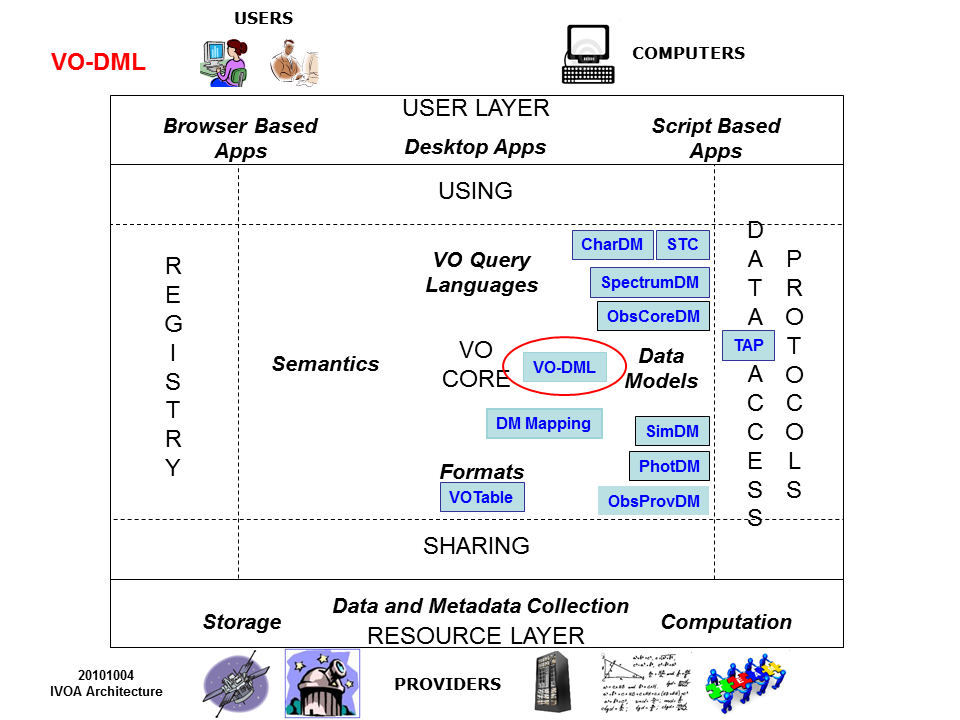
\includegraphics[width=6in,height=4.5in]{./media/image3.png}

Note that in the diagram not all existing DMs are represented. This
specification \emph{is} supposed to apply to all models.

\hypertarget{data-integration}{%
\section{\texorpdfstring{Data Integration
}{Data Integration }}\label{data-integration}}

The home page of the IVOA web site states that:

\emph{The Virtual Observatory (VO) is the vision that astronomical
datasets and other resources should work as a seamless
whole.}\footnote{http://www.ivoa.net/}

While Wikipedia states that:

\emph{\textbf{Virtual observatory} (VO) is a collection of
interoperating data archives and software tools which utilize the
internet to form a scientific research environment in which astronomical
research programs can be conducted.}

These characterizations of the VO are very similar to the various
definitions of \emph{data integration} one encounters when searching the
web, such as

\emph{\textbf{Data integration} involves combining data residing in
different sources and providing users with a unified view of these
data.}\footnote{\url{http://en.wikipedia.org/wiki/Data_Integration}}

\emph{\textbf{Data integration} involves combining data from several
disparate sources, which are stored using various technologies and
provide a unified view of the data}\footnote{\url{http://www.dataintegration.info/data-integration}}\emph{.}

And from Chapter 9 in {[}1{]}, which we will use in much of this
introduction

\emph{The goal of data integration is to provide a uniform access to a
set of autonomous and possibly heterogeneous data sources in a
particular application domain.}

In fact, the Virtual Observatory can be seen as what {[}1{]} calls a
\emph{virtual} data integration effort: the data remain in their data
sources; the integration is performed only when the data is needed, say
during a query. The unified view of the data in such data integration
projects is provided by what is commonly called a \emph{global schema}.
The global schema aims to represent, in a unified view, the information
contained in the source databases pertaining to a certain domain, or
\emph{universe of discourse}.

The goal of data integration projects such as the VO is to provide end
users with a view of the source databases based on this schema. For
example, users could be allowed to submit queries phrased in terms of
this schema rather than in terms of the schemas of the underlying
databases. Or serialized data sets should be expressed using terms of
the global schema. Or it should be possible to write code against
programming APIs designed according to the global schema.

The central problem of both IVOA and data integration in general is that
the source databases generally do not conform to any common schema one
might wish to design. The source databases have generally been created
to serve the purposes of the entity/organization that owns them, without
coordination between the different providers to align their designs.
This shows itself in two ways: First is what one might call
\emph{technical heterogeneity}; source databases are built using
different technologies or use different formats. Experience in the VO
shows that this can be solved: owners of the data are willing to
describe their data holdings in some standardized format and abide by
some standard access protocols (e.g. TAP), or send their data over the
net in some standardized serialization format (e.g. VOTable).

What is much harder to solve and is the target of the current work as
well as the related \emph{Mapping to VOTable} specification {[}3{]}, is
what is called in {[}1{]} \emph{semantic heterogeneity}. Source
databases contain information from possibly overlapping but not
identical subsets of the whole problem domain, and even where there is
overlap in contents, the design will generally be different. The source
databases were generally built according to local specifications,
targeting different subsets of the overall domain (Astronomy for the
VO), and the designs use particular \emph{views} of the schema optimized
for particular applications and/or implementations.

So even if all source databases are relational, the actual data models
they use are different and data providers will in general be unwilling
or unable to change the structural design of their data holdings, or the
contents of the serializations, to conform to some uniform, global
design. Instead a mapping must be provided between the source schemas
and the global schema. In the literature the components providing this
mapping are often referred to as \emph{mediators}.

The link between the global schema and the various \emph{data models}
defined in the IVOA is easy to see. Similar to global schemas, data
models in the IVOA have a particular goal, namely to facilitate
interoperability of distributed data sources. They can provide
serialization formats for the results of protocols such as the spectrum
data model in SSAP {[}23{]} or can provide a common relational schema as
in ObsCore+ObsTAP {[}24{]}.

\emph{Mediators} are not as easily identified or isolated, but they must
be hidden somewhere inside the different implementations of the various
IVOA access protocols. For example in an implementation of SSAP a
special code component may translate some native representation of a
spectrum into one of the few allowed forms allowed by the protocol. And
in ObsTAP one may be able to define database views on the native schema
to represent the ObsCore table(s).

The two examples mentioned above, SpectrumDM+SSAP and ObsCore+ObsTAP,
are not the only, or even most common data integration patterns in the
IVOA. What distinguishes these from other approaches is that a data
model is represented \emph{faithfully}, i.e. the protocol serializations
produced by the protocol, or the database design exposed by the data
providers, is basically a one-to-one representation of the common data
model defined by the standard. Especially ObsTAP is a nice example of a
pattern that is equivalent to the data integration pattern called
\emph{global-as-view}. The global schema can sometimes literally be
implemented as a collection of database views on the source schemas.
These views show \emph{how} the entities from the global schema are
represented in \emph{and} how they can be extracted from the source
database\footnote{For the use of the view concept in data and
  information integration see {[}2{]}.}.

In the IVOA this pattern is still rare. The more common way by which one
may obtain knowledge about the contents of some data source in
standardized terms is through \emph{annotations}. Data sets are
represented in some standardized format that includes hooks for
associating terms from a standardized source of semantic information. In
the IVOA the main representations that allow this are the metadata
annotation elements in VOTable {[}4{]} and the TAP\_SCHEMA\footnote{Note,
  in this document, we use the term TAP\_SCHEMA for the way metadata
  about a TAP service is represented, not necessarily only about the
  actual TAP\_SCHEMA tables.} in the TAP specification {[}5{]}. Each of
these contains hooks for linking certain data components to the UCD
semantic vocabulary (see {[}6{]} and {[}7{]}). Associating a term from
that controlled list to say a FIELD (VOTable) or column (TAP) indicates
that those elements represent the concept identified by the term.

It was recognized that apart from the controlled vocabularies, also the
various data models defined for varying purposes within the IVOA contain
semantic information. Maybe it would be possible to provide a mechanism
similar to the UCD annotations that would allow one to associate
elements from a data source with elements inside these models. The
\emph{utype} attribute was defined in VOTable to represent such
"pointers into a data model".

What these were supposed to point at was left unspecified in the VOTable
specification, the current specification provides that definition. This
specification defines a formal language for defining IVOA data models.
Data models defined in this language contain explicitly identified data
model elements that can be formally referenced using a namespace-like
mechanism for avoiding name clashes among different Data
Models.\footnote{Note that a separate specification is in preparation to
  define how precisely to \emph{map} data models to VOTables. That
  specification does actually \emph{not} use the utype attribute, but
  introduces a new \textless VODML\textgreater{} element that is more
  expressive and tuned to the VO-DML language.}

The language defined here is called \emph{VO-DML}, which stands for
\emph{Virtual Observatory Data Modeling Language}. VO-DML is designed to
satisfy the following requirements. It should

\begin{enumerate}
\def\labelenumi{\arabic{enumi}.}
\item
  Support the specification of serialization strategies for serializing
  instances of data models into different file formats;
\item
  Be rich enough to represent existing IVOA data models;
\item
  Support model reuse;
\item
  Be implementation-neutral, but...
\item
  Be flexible enough to be mapped to important physical representations,
  in particular XML schema, relational model (TAP), object-oriented
  languages (Java, Python...), and at the same time...
\item
  Be as minimal as possible, avoiding redundancy, adding restrictions
  where possible, with the aim of simplifying the work of modelers by
  offering few and ``obvious'' choices;
\item
  Be based on accepted standards for data modeling, but ...
\item
  Not \emph{rely} on external modeling tools\footnote{In particular
    graphical UML tools such as Modelio, MagicDraw or Altova Umodel.},
  but be sufficiently compatible with them so that such tools MAY be
  used when representing models;
\item
  Support runtime model interpretation;
\end{enumerate}

The data modeling language defined in this document fulfills these
requirements.

The language is explicitly implementation neutral, but has been
successfully used as the source for transformation scripts that produce
various representations such as a fully hyper-linked HTML document and
Java classes used to infer data model instances form suitably mapped
VOTables\footnote{This work again is not complete, but an earlier
  version of VO-DML was used to generate XSD and RDB representations
  used in proof-of-concept implementations for the the Simulation Data
  model specification{[}8{]}. which gave rise to the VO-URP framework to
  generate a complete set of representations.}. The formal
representation language is XML that can be easily hand coded, but also
has a non-normative UML ({[}12{]}, {[}13{]}) representation that can be
translated into VO-DML automatically. Finally the model representation
language can be used in validating VOTables annotated using vodml-ids.

Applications making use of VO-DML XML descriptions can be agnostic of
the actual models, but can successfully retrieve, parse and load those
at runtime.

The VO-DML specification consists of a conceptual part and a model
definition language. The latter defines an XML format and this
specification states that all data models in the IVOA MUST have a
representation in that format. The conceptual part of the spec goes by
the name of \textbf{VO-DML}, short for VO Data Modeling Language. The
serialization language goes by the name of \textbf{VO-DML/Schema} and an
XML document conforming to this standard defines a data model, and is
referred to as the \textbf{VO-DML/XML} representation of that data
model.

The language can be expressed graphically using a subset of UML. For
this purpose a UML Profile\footnote{http://www.uml-diagrams.org/profile-diagrams.html}
is defined that represents the VO-DML concepts in UML. This is referred
to as \textbf{VO-UML}, but its definition is \emph{informative},
\emph{not} a normative part of the spec. These four different
representations will be discussed in more detail in the next section.
Section 3 then defines each modeling concept in detail and illustrates
their usages in the different representations. Section 4 defines
normative rules how to define data models in the IVOA and gives some
non-normative \emph{best practices} guide lines. Auxiliary material is
contained in the appendices.

\hypertarget{vo-dml-vo-uml-vo-dmlschema-and-vo-dmlxml}{%
\section{\texorpdfstring{VO-DML, VO-UML, VO-DML/Schema and\\
VO-DML/XML}{VO-DML, VO-UML, VO-DML/Schema and VO-DML/XML}}\label{vo-dml-vo-uml-vo-dmlschema-and-vo-dmlxml}}

This specification distinguishes between the conceptual meta-model,
\textbf{VO-DML} and the XML based serialization language for expressing
data models, referred to as \textbf{VO-DML/XML}. The latter is defined
using an XML schema together with a Schematron\footnote{http://www.schematron.com/}
file defining further constraints and is referred to in combination as
\textbf{VO-DML/Schema}. The relation between VO-DML and VO-DML/XML is
equivalent to the relation between a UML {[}12{]} (see also {[}16{]})
model and its representation as a file in the XML serialization format
XMI {[}15{]}\emph{.} VO-DML is directly derived from UML in the sense
that most of its modeling constructs have a counterpart in UML. One can
in fact interpret VO-DML as a UML \emph{Profile} {[}16{]}, a domain
specific "dialect" of UML. This is made explicit in this specification
by providing a (non-normative) UML representation of VO-DML, referred to
as \textbf{VO-UML}.

These different components of the specification are discussed in some
more detail in the next subsections.

\hypertarget{vo-dmlxml-vo-dmlschema}{%
\subsection{VO-DML/XML + VO-DML/Schema}\label{vo-dmlxml-vo-dmlschema}}

For most use cases a VO-DML data model must be serialized in a computer
readable format. The serialization language to be used for this is
referred to as VO-DML/XML. A VO-DML/XML document is an XML document that
must conform to a formal syntax defined by an XML schema\footnote{XML
  Schema was chosen as the core language for VO-DML/XML, as it was felt
  it is more familiar to the IVOA community than Schematron.},
vo-dml.xsd\footnote{\url{http://www.ivoa.net/xml/VODML/vo-dml-v1.xsd}}
and must further validate under the rules defined in an associated
Schematron file, vo-dml.sch.xml\footnote{\url{http://www.ivoa.net/xml/VODML/vo-dml-v1.sch.xml}}.
These files implement all the concepts described in section 4 The schema
files are self-documented as much as possible, and in what follows only
a few details of the overall design, focusing on technical aspects of
the implementation, are given.

VO-DML/XML is a simple representation of a VO-DML model as an XML
document. The fact that this specification defines a custom designed
serialization language rather than using some existing language could be
seen as an unnecessary complication. One \emph{could} for example also
consider using XMI as the standard for serializing VO-DML models.
However, XMI is a rather unwieldy format that hides many of the features
that are made explicit in this specification. Hence as a language from
which to derive information of the model without very sophisticated
tools it is ill-suited. Also one should not assume all users have access
to a UML modeling tool that can support all the UML modeling features
needed to create VO data models, and hand-editing XMI is nigh
impossible. It is also foreseen that users may want to derive models
from other representations (e.g. XML schema, or RDF) and XMI as target
language for such a tool requires deep understanding of its format,
which is not necessary for the simple language proposed here.

VO-DML/XML is a useful language for serializations, in particular
because, being completely under control of the IVOA DM WG, it can be
tailored to the requirements deriving from its usage in the IVOA. This
provides more freedom to restrict the format and implement the
appropriate constraints. This is formal in the sense that VO-DML/XML
files MUST conform to these specifications. The implementation of VO-DML
provided by these files is referred to as VO-DML/Schema. VO-DML/Schema
is a direct implementation of the VO-UML profile: it exposes all
modeling concepts explicitly, and ignores the many UML/XMI features that
are not needed.

\hypertarget{vo-dml-vo-uml}{%
\subsection{VO-DML + VO-UML}\label{vo-dml-vo-uml}}

VO-DML defines the concepts used to create data models in the IVOA. It
uses a small subset of the components from UML Class Diagrams\footnote{All
  formal references are to version 2.4.1 of the UML spec, though the
  components used in VO-DML are standard since at least version 2.0.}
and hence follows an object-oriented approach. VO-DML restricts itself
to structural constructs only; operations are explicitly excluded from
our language. Constraints are supported, but in a very limited manner.

A great strength of UML is its formal graphical language and though only
a VO-DML/XML representation of a model will be required for IVOA data
models, human-readable graphical representations are extremely useful to
interpret and understand a model. Until a graphical VO-DML tool exists,
modelers can use one of the many available UML modeling tools to create
such a representation.

VO-UML has been expressed at least in one such UML modeling tool as a
UML \emph{profile}, using \emph{stereotypes} with \emph{tag definitions}
to enable modeling of domain specific components in the graphical tool
and to facilitate automated generation of VO-DML/XML from the XMI in
which the UML model was serialized.

But note, though VO-UML is used for illustrations, and has been used to
define some models, the VO-DML specification is \emph{not dependent} on
UML or any tools for defining models in UML. VO-DML data models need not
have a UML representation, but they MUST have a serialization in terms
of VO-DML/XML (see section 5 for details on how to define data models).
Hence the VO-UML part in this spec is INFORMATIVE, not NORMATIVE. But if
a UML representation is provided, it SHOULD restrict oneself to those
UML elements that match the VO-DML concepts as defined in this
specification. This will further facilitate the application of tools for
generating VO-DML/XML from the UML directly.

\hypertarget{this-specification}{%
\subsection{\texorpdfstring{This specification
}{This specification }}\label{this-specification}}

Section 4 defines all the major components of the VO-DML meta-model.
Each subsection defines a concept in its title and contains a
description of its meaning at the conceptual, VO-DML level. In
appropriately titled sub-sub-sections it lists and describes all the
sub-components.

As the VO-DML modeling language can be interpreted as a subset of the
UML modeling language, this document is basically a listing of those UML
components that are part of the language with a description how they are
used, restricted and in some cases renamed. This link is made explicit
in the sections headed with the phrase \textbf{VO-UML}. Those sections
identify the UML concepts, or \emph{meta-class}, from UML version 2.4.1
{[}13{]} that is closest in meaning to the VO-DML concept and provide
hyperlinks to the rather more readable UML Diagrams website {[}16{]}.

Where appropriate\footnote{Not all UML concepts have a graphical
  representation.} the \textbf{VO-UML} section also contains a sample
graphical representation of the concept using snippets from a sample UML
model described in Appendix D. This is a toy data model for astronomical
Source-s and is designed specifically to illustrate most of the modeling
constructs. See the appendix for details on where its different
representations can be found. The diagrams for this model were created
using a particular UML modeling tool (MagicDraw Community Edition 12.1).
This version supports UML 2.0\footnote{\url{http://schema.omg.org/spec/UML/2.0}.
  The graphical elements are available in both UML 2.0 and 2.4.1, but
  MagicDraw CE 12.1 only supported 2.0.}, serializing its models to XMI
2.1\footnote{http://schema.omg.org/spec/XMI/2.1.}. An explicit UML
\emph{Profile}\footnote{See
  http://www.uml-diagrams.org/profile-diagrams.html\#profile} was
created to represent also those VO-DML concepts that do not have a
direct UML counterpart. This Profile contains definitions for
stereotypes with tags that allow us to extend the definition of certain
UML elements so that these \emph{can} be directly mapped to VO-DML.

Applications aiming to automate generation of a VO-DML/XML
representation directly from the UML model may benefit from this
Profile. They may, for example, use the XMI serialization of the UML
model as source for an XSLT script. UML modeling tools may support a
similar Profile-based approach, or may have to use different means by
which to capture those VO-DML concepts that do not directly map to the
UML version they support\footnote{It should once more be made clear that
  the current spec \emph{does not} mandate the use of some particular
  UML modeling tool. But a UML representation different from VO-UML MUST
  NOT be used to define an IVOA data model \emph{without} an explicit
  mapping to VO-DML.}.

This graphical representation of VO-UML is \emph{not} normative, but
modelers are strongly urged that \emph{if} they use UML to illustrate
their models they use its design principles in constructing the
diagrams. In particular they should have a mapping from VO-DML concepts
to UML and obey the constraints implied by this mapping\footnote{E.g. as
  VO-DML does not allow multiple inheritance, the UML diagrams should
  not use this feature either.}.

In spite of its relation to UML, ultimately VO-DML should be expressed
in a VO-DML/XML document conforming to the formal VO-DML/Schema
documents.

This specification document can therefore also be seen as an explanation
of those documents. Each VO-DML concept listed in the next section has a
counterpart in the schema, which is replicated in shortened form in the
section headed with the term \textbf{VO-DML/SCHEMA}. The full definition
can be found in the corresponding schema documents that accompany this
specification. To repeat, this schema \emph{is} normative. I.e. all
models compliant to the VO-DML standard MUST be defined by a VO-DML/XML
document, which MUST conform to the schema and schematron files, as well
as by any rules and constraints written in the current document that may
not have been implemented explicitly in the schema.

Most subsections will also contain a section headed \textbf{VO-DML/XML},
which contains an example XML snippet extracted from the VO-DML/XML
representation of the sample model in Appendix D.

The fact that different representations of VO-DML are used, sometimes in
the same sentences, could make it difficult to understand which
representation one is referring to when using a named concept. In an
attempt to prevent this, the following notation is used to indicate
which representation is intended: references referring to a VO-DML
\emph{concept} are in \textbf{boldface}; references to an XML schema
implementation of a concept are in courier font; references to a UML
concept are in \emph{italics}.

\hypertarget{vo-dml-language-specification-normative}{%
\section{VO-DML Language Specification
{[}NORMATIVE{]}}\label{vo-dml-language-specification-normative}}

This section defines all the elements from the VO-DML meta-model. The
order in which the elements appear is roughly based on a dependency
hierarchy between the meta-elements, which is visualized in the diagram
in Figure 1. That diagram shows a representation of the VO-DML
meta-model as a UML-like diagram. It leaves out most of the details,
focusing on the inheritance hierarchy between the meta-model concepts
represented by the boxes. This diagram is inspired by the first diagram
in {[}18{]}, which shows the components of the Ecore meta-model used in
the Eclipse Modeling Framework\footnote{\url{https://www.eclipse.org/modeling/emf/}}.

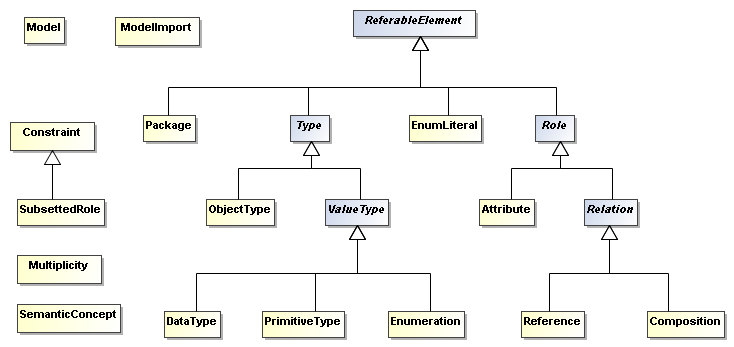
\includegraphics[width=6in,height=2.83302in]{./media/image4.png}

Figure : UML-like diagram of the main components of the VO-DML
meta-model.

More detailed diagrams are shown in Figure 2 and Figure 3. These
diagrams also show the attributes and non-inheritance relations between
the concepts. Note that these diagrams are not VO-UML diagrams and
certain rules of VO-DML are not obeyed here\footnote{For example
  Attribute is contained by both ObjectType \emph{and} DataType and
  Package contains itself. As this meta-model is not supposed to be a
  model of a data structure, but of a language, and moreover since the
  diagram is meant for illustration only, this should not give rise to
  confusion.}. It is purely meant to illustrate the meta-model and allow
comparison with the similar diagrams in the \emph{Ecore} meta-model in
{[}18{]}.

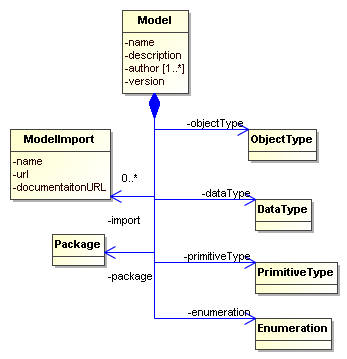
\includegraphics[width=3.61458in,height=3.73958in]{./media/image5.png}

Figure : The structure of a Model, consisting of packages, various types
and possibly imported models.

The subsections in this chapter have titles that name the concepts.
Abstract elements have a slanted title. Child components have in general
a title that follows the name of the element, separated by a colon.
References to other elements are implemented as much as possible using
hyperlinks. When primitive types are needed, the names from the basic
"IVOA" data model introduced in section 5 are used. These names are
common and the model is not really required to understand their meaning.
Ultimately the XSD representation of each element is normative and it
uses the standard set of primitive types such as xsd:string etc.

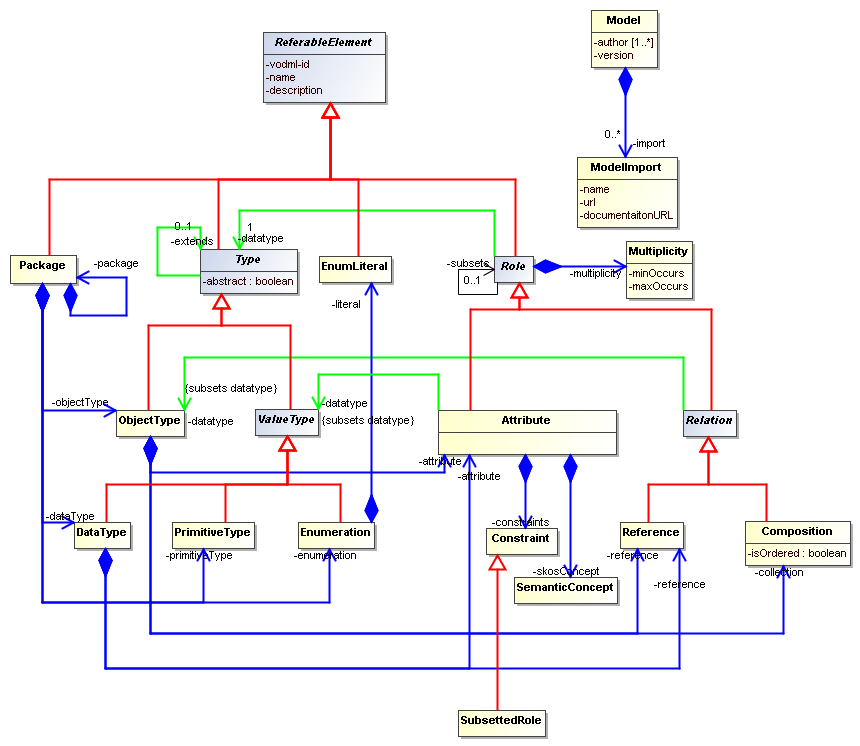
\includegraphics[width=6.42681in,height=5.57037in]{./media/image6.png}

Figure Detailed view of the meta-model hierarchy below
\emph{ReferableElement}. Composition and reference relation are
indicated as well as attributes.

\hypertarget{referableelement}{%
\subsection{\texorpdfstring{\emph{ReferableElement}
}{ReferableElement }}\label{referableelement}}

A data model consists of model elements of various types. In the
VO-DML/XML serialization almost all of these MUST have an explicit
identifier element that makes it possible for them to be explicitly
referenced, either from inside the model, or from an external context.
VO-DML/Schema defines the abstract type ReferableElement that is a
super-type of all types representing such referable concepts. It
contains an identifier element named vodml-id that MUST be unique within
the model.

Note that for convenience vodml-id SHOULD be human-readable, following
to the grammar defined in Appendix C. While this is not obligatory,
since vodml-ids are only required to be unique in a model, it is
convenient for a human confronted by such an identifier to intuitively
infer its meaning. Following a standard grammar improves consistency
among data models.

All referable elements also have a \textbf{name}, and a
\textbf{description}. The name SHOULD be used to derive the vodml-id
from the structure of the model, as described in Appendix C.

The name must often be unique within the direct context where a
particular referable element is defined. For example all \textbf{Types}
defined as direct children of a \textbf{Package} must have a name that
is unique in the context of that package. Similarly \textbf{Attributes}
must be unique in the definition of the \textbf{Type} they are defined
in; in fact this must be true for the whole collection of \textbf{Roles}
in the inheritance hierarchy of the type.

VO-UML

Closest UML meta-class:
\href{http://www.uml-diagrams.org/uml-core.html\#named-element}{\emph{NamedElement}}.
{[}§7.3.34 in {[}13{]}\footnote{The reference to the UML specification
  {[}13{]} will be left out from now on.}{]}.

\textbf{ReferableElement} does not have its own graphical element, but
has a representation in VO-UML as the stereotype
\textless\textless modelelement\textgreater\textgreater. That stereotype
defines a tag 'vodml-id'. When assigning the stereotype to a particular
model element one \emph{can} define an explicit value for the vodml-id
of the element, rather than the default value that is the one generated
from the VO-UML itself using the grammar described in Appendix C below.
In spite of this possibility, modelers SHOULD NOT define custom
vodml-id, as the grammar offers an explicit, human readable expression
that gives some hints as to the location of the element in the model.
The main reason to do so is to use values from old lists of utype-s for
example.

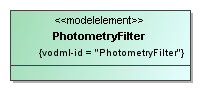
\includegraphics[width=1.66667in,height=0.75in]{./media/image7.png}

Figure VO-UML type with an explicit
\textless\textless modelelement\textgreater\textgreater{} stereotype.
This allows one to explicitly assign a vodml-id, possibly overriding the
one that would be automatically assigned using the algorithm in Appendix
C.

VO-DML/Schema

All main modeling elements in the VO-DML XSD (apart from Model) extend
ReferableElement. This abstract base class has an identifier element
\textless vodml-id\textgreater, the value of which must be unique in the
model. This means that these elements can be referenced using this
identifier. In VO-DML this is used explicitly in the ElementRef type
that expresses such references inside the meta-model using a
\textless vodml-ref\textgreater{} element. The type definitions for
vodml-id is that of a restricted string, the details of which are
expressed in the following XML Schema snippet.

\textless xsd:simpleType name=\emph{"VODMLID"} \textgreater{}

\textless xsd:restriction base=\emph{"xsd:string"}\textgreater{}

\textless xsd:pattern
value=\emph{"{[}}a-zA-Z\emph{{]}{[}}a-zA-Z0-9\_\textbackslash.{]}*\emph{"}/\textgreater{}

\textless/xsd:restriction\textgreater{}

\textless/xsd:simpleType\textgreater{}

\textless xsd:complexType name="ReferableElement"
abstract="true"\textgreater{}

\textless xsd:sequence\textgreater{}

\textless xsd:element name="vodml-id" type="VODMLID"
minOccurs="1"/\textgreater{}

\textless xsd:element name="name" type="xsd:string"
minOccurs="1"/\textgreater{}

\textless xsd:element name="description" type="string"
minOccurs="0"/\textgreater{}

\textless/xsd:sequence\textgreater{}

\textless/xsd:complexType\textgreater{}

VO-DML/XML

As ReferableElement is abstract, there are no direct examples of its
usage, only through types derived from it.

\hypertarget{vodml-id-vodmlid-1}{%
\subsubsection{vodml-id : VODMLID {[}1{]}}\label{vodml-id-vodmlid-1}}

Identifier for the containing model element. Syntax in VO-DML/XML
defined by the VODMLID type, as shown in the VO-DML/Schema snippet
below.\\
This element MUST be formatted according to the regular expression in
the XML schema:

\begin{quote}
{[}a-zA-Z{]}{[}a-zA-Z0-9\_\textbackslash.{]}*
\end{quote}

The value assigned to an element MUST be unique in the document and is
case sensitive.

\hypertarget{name-xsdncname-1}{%
\subsubsection{name : xsd:NCName {[}1{]}}\label{name-xsdncname-1}}

The name of the model element. The name MUST conform to the following
XML Schema pattern defined in the VO-DML/XSD:

\begin{quote}
{[}a-zA-Z{]}{[}a-zA-Z0-9\_{]}*
\end{quote}

Names are often restricted by uniqueness constraints in subclasses of
\textbf{ReferableElement}. For examples names of \textbf{Types} must be
unique within their containing \textbf{Package}, \textbf{Role} names
must be unique within their containing \textbf{Type} etc.

\hypertarget{description-string-0..1}{%
\subsubsection{description : string
{[}0..1{]}}\label{description-string-0..1}}

Human readable description of the model element. Note the multiplicity
constraints. In principle every model element SHOULD have a meaningful
description, but no tool will be able to check whether a certain
description is correct. Since a meaningless string can easily be
provided if one wants to evade a possible not null constraint, the
description may be null.

\hypertarget{elementref}{%
\subsection{ElementRef}\label{elementref}}

To refer to a \protect\hyperlink{referableelement}{ReferableElement}
from inside a VO-DML/XML data model document, for example to indicate
the data type of an
\protect\hyperlink{attribute-extends-role}{\textbf{Attribute}} or other
\protect\hyperlink{role-extends-referableelement}{\textbf{Role}}, one
must use an ElementRef. This contains a single element named vodml-ref,
the value of which MUST be the exact vodml-id of the referenced element
(which MUST of course exist), is case-sensitive, and MUST be prefixed by
the name of the model the referenced element belongs to. This can be the
same model as the one containing the referencing element, or it may be a
model \protect\hyperlink{modelimport}{imported} by the current model.

VO-UML

This type has not explicit counterpart in VO-UML, though XMI's xmi:idref
is similarly playing the role of referring to other elements in the
model. In VO-DML, \textbf{ElementRef}-s may refer to elements defined in
an external, imported model without explicit representation in the model
that uses the type.

VO-DML/Schema

\textless xsd:simpleType name=\emph{"VODMLREF"}\textgreater{}

\textless xsd:restriction base=\emph{"xsd:string"}\textgreater{}

\textless xsd:pattern

value=\emph{"{[}a-zA-Z{]}{[}a-zA-Z0-9\_\textbackslash-{]}*:{[}a-zA-Z{]}{[}a-zA-Z0-9\_\textbackslash-\textbackslash.{]}*"}/\textgreater{}

\textless/xsd:restriction\textgreater{}

\textless/xsd:simpleType\textgreater{}

\textless xsd:complexType name=\emph{"ElementRef"}\textgreater{}

\textless xsd:sequence\textgreater{}

\textless xsd:element name=\emph{"vodml-ref"}
type=\emph{"VODMLREF"}\textgreater{}

\textless/xsd:element\textgreater{}

\textless/xsd:sequence\textgreater{}

\textless/xsd:complexType\textgreater{}

VO-DML/XML

Any usage of one type by another type, be it as data type of an
attribute, or as target type of a relation, will give rise to an
ElementRef definition in the corresponding VO-DML/XML. This generally
just means the element contains a \textless vodml-ref\textgreater{}
element that must conform to the syntax in the schema as in the
following example.

...

\textless datatype\textgreater{}

\textless vodml-ref\textgreater ivoa:string\textless/vodml-ref\textgreater{}

\textless/datatype\textgreater{}

...

See many more examples further on in this specification.

\hypertarget{vodml-ref-string-1}{%
\subsubsection{vodml-ref : string {[}1{]}}\label{vodml-ref-string-1}}

The element identifying the referenced target element. The syntax of the
vodml-ref consists of the name of the model, a colon ':' and the
vodml-id of the referenced element. In mock BNF:

\textless vodml-ref\textgreater{} :== \textless model-name\textgreater{}
':' \textless vodml-id\textgreater{}

\hypertarget{package-extends-referableelement}{%
\subsection{\texorpdfstring{Package extends
\protect\hyperlink{referableelement}{\emph{ReferableElement}}}{Package extends ReferableElement}}\label{package-extends-referableelement}}

\textbf{Packages} divide the set of types in a model in subsets that are
semantically related\footnote{\url{http://www.uml-diagrams.org/package-diagrams.html\#package}},
providing these with a common namespace: their names must be unique in
this context only. A package may contain child packages. This concept is
similar to for example an XML namespace, a Java package or a schema in a
relational database.

A package uses explicit element names for each of the type classes:
\textless objectType\textgreater,
\textless datatype\textgreater,\textless primitiveType\textgreater{} and
\textless enumeration\textgreater. This avoids the need for xsi:type
casting in serializations and facilitates tracing path expressions.

VO-UML

UML meta-class:
\href{http://www.uml-diagrams.org/package-diagrams.html\#package}{\emph{Package}}
{[}§7.3.38{]}

The graphical representation of a Package in UML is a tabbed rectangle
with name in the top of the rectangle as shown in Figure 5. Types owned
by the package may be shown inside the rectangle. Types may also have
the package name placed within parentheses below the name of the type.
See the Source type in the figure for an example of the latter.

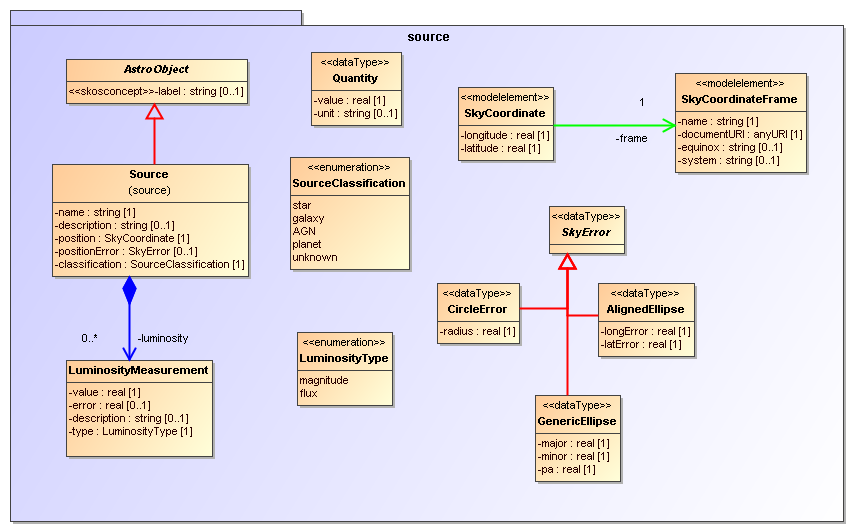
\includegraphics[width=6in,height=3.72222in]{./media/image8.png}

Figure A package is represented by a tabbed rectangle. Types belonging
to it can be drawn inside it.

\textbf{VO-DML/Schema}

In VO-DML/Schema, \textbf{Package} is represented by a complexType of
the same name and extends ReferableElement.

\textless xsd:complexType name=\emph{"Package"}\textgreater{}

\textless xsd:complexContent\textgreater{}

\textless xsd:extension base=\emph{"ReferableElement"}\textgreater{}

\textless xsd:sequence\textgreater{}

\textless xsd:element name=\emph{"objectType"} type=\emph{"ObjectType"}
minOccurs=\emph{"0"}

maxOccurs=\emph{"unbounded"/}\textgreater{}

\textless xsd:element name=\emph{"dataType"} type=\emph{"DataType"}
minOccurs=\emph{"0"}

maxOccurs=\emph{"unbounded"/}\textgreater{}

\textless xsd:element name=\emph{"enumeration"}
type=\emph{"Enumeration"}

minOccurs=\emph{"0"} maxOccurs=\emph{"unbounded"/}\textgreater{}

\textless xsd:element name=\emph{"primitiveType"}
type=\emph{"PrimitiveType"}

minOccurs=\emph{"0"} maxOccurs=\emph{"unbounded"/}\textgreater{}

\textless xsd:element name=\emph{"package"} type=\emph{"Package"}
minOccurs=\emph{"0"}

maxOccurs=\emph{"unbounded"/}\textgreater{}

\textless/xsd:complexContent\textgreater{}

\textless/xsd:extension\textgreater{}

\textless/xsd:complexType\textgreater{}

\textbf{VO-DML/XML}

\textless package\textgreater{}

\textless vodml-id\textgreater source\textless/vodml-id\textgreater{}

\textless name\textgreater source\textless/name\textgreater{}

\textless description\textgreater...\textless/description\textgreater{}

\textless objectType\textgreater{}

\textless vodml-id\textgreater source.LuminosityMeasurement\textless/vodml-id\textgreater{}

\textless name\textgreater LuminosityMeasurement\textless/name\textgreater{}

...

\hypertarget{objecttype-objecttype-0..}{%
\subsubsection{\texorpdfstring{objectType :
ObjectType\textsuperscript{{[}\protect\hyperlink{objecttype-extends-type}{→}{]}}
{[}0..*{]}}{objectType : ObjectType{[}→{]} {[}0..*{]}}}\label{objecttype-objecttype-0..}}

Collection of ObjectTypes defined in this package.

\hypertarget{datatype-datatype-0..}{%
\subsubsection{\texorpdfstring{dataType :
DataType\textsuperscript{{[}\protect\hyperlink{datatype-extends-valuetype}{→}{]}}
{[}0..*{]}}{dataType : DataType{[}→{]} {[}0..*{]}}}\label{datatype-datatype-0..}}

Collection of DataTypes defined in this package.

\hypertarget{primitivetype-primitivetype-0..}{%
\subsubsection{\texorpdfstring{primitiveType :
PrimitiveType\textsuperscript{{[}\protect\hyperlink{_Type_extends_ReferencableElement}{→}{]}}
{[}0..*{]}}{primitiveType : PrimitiveType{[}→{]} {[}0..*{]}}}\label{primitivetype-primitivetype-0..}}

Collection of PrimitiveTypes defined in this package.

\hypertarget{enumeration-enumeration-0..}{%
\subsubsection{\texorpdfstring{enumeration :
Enumeration\textsuperscript{{[}\protect\hyperlink{enumeration-extends-valuetype}{→}{]}}
{[}0..*{]}}{enumeration : Enumeration{[}→{]} {[}0..*{]}}}\label{enumeration-enumeration-0..}}

Collection of Enumerations defined in this package.

\hypertarget{package-package-0..}{%
\subsubsection{\texorpdfstring{package :
Package\textsuperscript{{[}\protect\hyperlink{package-extends-referableelement}{→}{]}}
{[}0..*{]}}{package : Package{[}→{]} {[}0..*{]}}}\label{package-package-0..}}

Collection of child packages defined in this package.

\hypertarget{model}{%
\subsection{Model}\label{model}}

A \textbf{Model} represents a complete data model. It represents a
coherent set of type definitions, by which it represents the concepts
that have an explicit place in its \emph{universe of discourse}, i.e.
the set of concepts one can talk/"discourse" about in the model's
context. In VO-DML each data model is defined in a single document, but
\textbf{Model} is an explicit concept\footnote{Rather than just the
  container of its content.} in VO-DML that is particularly important
for supporting model reuse through the \textbf{import} feature (see
4.4.10).

Note that although the vodml-id of model elements MUST NOT have the
prefix, references from model elements to other elements inside the same
model MUST use the full vodml-ref definition 4.2.1 , i.e. MUST include
the model's name as prefix.

\textbf{Model} has the following components, which have a 1-1
correspondence in the VO-DML/Schema. See there for more extensive
comments.

VO-UML

Derived from UML element:
\href{http://www.uml-diagrams.org/package-diagrams/model.html}{\emph{Model}}
{[}§17.3.1{]}.

In UML a Model\footnote{http://www.uml-diagrams.org/package-diagrams/model.html}
is a special kind of Package and is represented by the package symbol
with a triangle in the top right as shown in Figure 6

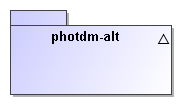
\includegraphics[width=1.53333in,height=0.86667in]{./media/image9.png}

Figure UML representation of a Model as a special kind of package.

In the Profile used for these diagrams the root of the document
represents the model and a separate graphical element is not
required\footnote{But see \protect\hyperlink{ModelImport}{ModelImport}.}.
The VO-UML profile contains a
\textless\textless model\textgreater\textgreater{} \emph{stereotype}
that can be assigned to a Model and which defines \emph{tags} which
allow one to define extra metadata about the model and which correspond
to the metadata elements defined in the subsections below.

\textbf{VO-DML/Schema}

In VO-DML/Schema \textbf{Model} is represented by a complexType Model.
It contains definitions for model specific meta-data elements.
\textbf{Model} is furthermore represented by the single root element
defined in the schema, named model. This has type Model and has a
uniqueness constraint defined on the
\protect\hyperlink{vodml-id-vodmlid-1}{vodml-id}-s of all its contained
elements.

\textless xsd:complexType name="Model"\textgreater{}

\textless xsd:sequence\textgreater{}

\textless xsd:element name="name" type="ModelName" minOccurs="1"

maxOccurs="1"/\textgreater{}

\textless xsd:element name="description" type="xsd:string" minOccurs="0"

maxOccurs="1"/\textgreater{}

\textless xsd:element name="identifier" type="xsd:string" minOccurs="0"

maxOccurs="1"/\textgreater{}

\textless xsd:element name="uri" type="xsd:anyURI" minOccurs="1"

maxOccurs="1"/\textgreater{}

\textless xsd:element name="title" type="xsd:string" minOccurs="1"

maxOccurs="1"/\textgreater{}

\textless xsd:element name="author" type="xsd:string" minOccurs="0"

maxOccurs="unbounded"/\textgreater{}

\textless xsd:element name="version" type="xsd:string"
minOccurs="1"/\textgreater{}

\textless xsd:element name="previousVersion" type="xsd:anyURI"

minOccurs="0"/\textgreater{}

\textless xsd:element name="lastModified"
type="xsd:dateTime"/\textgreater{}

\textless xsd:element name="import" type="ModelImport" minOccurs="0"

maxOccurs="unbounded"/\textgreater{}

\textless xsd:element name="package" type="Package" minOccurs="0"

maxOccurs="unbounded"/\textgreater{}

\textless xsd:element name="objectType" type="ObjectType" minOccurs="0"

maxOccurs="unbounded"/\textgreater{}

\textless xsd:element name="dataType" type="DataType" minOccurs="0"

maxOccurs="unbounded"/\textgreater{}

\textless xsd:element name="enumeration" type="Enumeration"
minOccurs="0"

maxOccurs="unbounded"/\textgreater{}

\textless xsd:element name="primitiveType" type="PrimitiveType"

minOccurs="0" maxOccurs="unbounded"/\textgreater{}

\textless/xsd:sequence\textgreater{}

\textless/xsd:complexType\textgreater{}

\textbf{VO-DML/XML}

\textless vo-dml:model
xmlns:vo-dml="http://www.ivoa.net/xml/VODML/v1"\textgreater{}

\textless name\textgreater src/name\textgreater{}

\textless description\textgreater This is a sample data model. ...

\textless/description\textgreater{}

\textless uri\textgreater http://ivoa.net/vodml/source1.vo-dml\textless/uri\textgreater{}

\textless title\textgreater Sample VO-DML data
model.\textless/title\textgreater{}

\textless version\textgreater0.x\textless/version\textgreater{}

\textless lastModified\textgreater2013-05-04T19:24:52\textless/lastModified\textgreater{}

\textless import\textgreater{}

\textless name\textgreater photdm-alt\textless/name\textgreater{}

\textless version\textgreater1.0\textless/version\textgreater{}

\textless url\textgreater https://volute.g-vo.org/svn/trunk/projects/dm/vo-dml/models/sample/filter/Filter.vo-dml.xml\textless/url\textgreater{}

\textless documentationURL\textgreater https://volute.g-vo.org/svn/trunk/projects/dm/vo-dml/models/sample/filter/Filter.html\textless/documentationURL\textgreater{}

\textless/import\textgreater{}

...

\hypertarget{name-string-1}{%
\subsubsection{name : string {[}1{]}}\label{name-string-1}}

The short name and identifier for this model. A standard model's
\emph{name} is assumed to be globally unique in the IVOA\footnote{See
  section 6 on registration of data models below for more details.}.
Model definitions that are not part of the IVOA standards but are
intended to extend a standard model SHOULD use the underscore character
and a unique prefix for their models, e.g. ``gaia\_src'' in order to
avoid name clashes with other extensions from other authors. The
name/identifier is also used as the prefix in the construction of
strings referencing the model with that name, e.g. ``src:Source''.

For its role as prefix in VODMLREFs we restrict the valid values of the
model name to the following XML Schema pattern (defined in the ModelName
type in the VO-DML/XSD):

\begin{quote}
{[}a-zA-Z{]}{[}a-zA-Z0-9\_\textbackslash-{]}*
\end{quote}

\hypertarget{description-string-0..1-1}{%
\subsubsection{description : string
{[}0..1{]}}\label{description-string-0..1-1}}

long description for the \textbf{Model}

\hypertarget{identifier-string0..1}{%
\subsubsection{identifier :
string{[}0..1{]}}\label{identifier-string0..1}}

A string holding the identifier by which the current model is registered
in an IVOA compatible registry. Its structure must therefore conform to
the IVOA Identifier specification {[}28{]}. If the model is an IVOA
standard, the naming authority for the identifier should be the IVOA DM
working group. See section 6 for more details on how data models are to
be registered.

\hypertarget{uri-anyuri-1}{%
\subsubsection{uri: anyURI {[}1{]}}\label{uri-anyuri-1}}

Each model has an associated model URI that MUST be used to reference
it, for example in \protect\hyperlink{modelimport}{ModelImports} or in
VOTable annotations. Dereferencing the model URI and following redirects
yields the latest VO-DML for the data model. In accordance to the
proposal in {[}29{]}, the model URI must not contain minor versions.
IVOA-approved data models will have URIs of the form

\url{http://ivoa.net/vodml/\%3cname\%3e.vo-dml},

where 'name' will already contain the major version (as in, for
instance, \emph{stc2}). The minor version of the model will be contained
in the \emph{version} attribute defined below.

Non-IVOA providers of VO-DML files should follow the IVOA practice of
returning a \emph{302 Found} redirect when dereferencing model URIs. The
URI redirected to should be stable for the exact version, including
minor and possibly micro releases, so that clients can easily determine
what actual file they are running against. This is primarily relevant
for debugging.

\hypertarget{title-string-1}{%
\subsubsection{title : string {[}1{]}}\label{title-string-1}}

Long name for the \textbf{Model}.

\hypertarget{author-string0..}{%
\subsubsection{author : string{[}0..*{]}}\label{author-string0..}}

List of names of authors who have contributed to this model.

\hypertarget{version-string-1}{%
\subsubsection{version : string {[}1{]}}\label{version-string-1}}

Label indicating the version of this model.

\hypertarget{previousversion-anyuri-0..1}{%
\subsubsection{previousVersion : anyURI
{[}0..1{]}}\label{previousversion-anyuri-0..1}}

URI identifying a VO-DML model that is the version from which the
current version of model is derived.

\hypertarget{lastmodified-datetime-1}{%
\subsubsection{lastModified : dateTime
{[}1{]}}\label{lastmodified-datetime-1}}

Timestamp when the last change to the current model was made.

\hypertarget{import-modelimport-0..}{%
\subsubsection{\texorpdfstring{import :
\protect\hyperlink{modelimport}{ModelImport}
{[}0..*{]}}{import : ModelImport {[}0..*{]}}}\label{import-modelimport-0..}}

An 'import' element indicates a dependency on an external, predefined
VO-DML data model. Types from that model may be referenced, extended, or
assigned to attributes as data types. Types from the external model MUST
NOT be used for composition relationships.

\hypertarget{package-package-0..-1}{%
\subsubsection{\texorpdfstring{package :
Package\textsuperscript{{[}\protect\hyperlink{package-extends-referableelement}{→}{]}}
{[}0..*{]}}{package : Package{[}→{]} {[}0..*{]}}}\label{package-package-0..-1}}

Collection of child packages defined in this model.

\hypertarget{objecttype-objecttype-0..-1}{%
\subsubsection{\texorpdfstring{objectType :
ObjectType\textsuperscript{{[}\protect\hyperlink{objecttype-extends-type}{→}{]}}
{[}0..*{]}}{objectType : ObjectType{[}→{]} {[}0..*{]}}}\label{objecttype-objecttype-0..-1}}

Collection of ObjectTypes defined directly under the model.

\hypertarget{datatype-datatype-0..-1}{%
\subsubsection{\texorpdfstring{dataType :
DataType\textsuperscript{{[}\protect\hyperlink{datatype-extends-valuetype}{→}{]}}
{[}0..*{]}}{dataType : DataType{[}→{]} {[}0..*{]}}}\label{datatype-datatype-0..-1}}

Collection of DataTypes defined directly under the model.

\hypertarget{enumeration-enumeration-0..-1}{%
\subsubsection{\texorpdfstring{enumeration :
Enumeration\textsuperscript{{[}\protect\hyperlink{enumeration-extends-valuetype}{→}{]}}
{[}0..*{]}}{enumeration : Enumeration{[}→{]} {[}0..*{]}}}\label{enumeration-enumeration-0..-1}}

Collection of Enumerations defined directly under the model.

\hypertarget{primitivetype-primitivetype-0..-1}{%
\subsubsection{\texorpdfstring{primitiveType :
PrimitiveType\textsuperscript{{[}\protect\hyperlink{_Type_extends_ReferencableElement}{→}{]}}
{[}0..*{]}}{primitiveType : PrimitiveType{[}→{]} {[}0..*{]}}}\label{primitivetype-primitivetype-0..-1}}

Collection of PrimitiveTypes defined directly under the model.

\hypertarget{modelimport}{%
\subsection{ModelImport}\label{modelimport}}

A \textbf{Model} can \textbf{import} (see 4.4.10) another
\textbf{Model}. This implies that elements of the imported
\textbf{Model} are used in the definition of elements in the current
\textbf{Model}. For example when Types from another model are assigned
to Roles, or when a Type inherits from a Type in another model, then
that model MUST be imported. In a VO-DML model document the imported
\textbf{Model} is represented by a \textbf{ModelImport} element that
contains metadata components identifying the remote model and its
documentation, as well as its name that must be used as prefix when
referring to elements in the imported model.

Note that only models that are directly used, or whose types are
extended must be imported. But model import is not transitive. For
example, if model A uses model B, and model B uses model C (but model A
does not), only model B must be imported in model A. But if model A
\emph{does} use elements from model C explicitly, than A MUST import
model C as well\footnote{One reason for this is that the ModelImport
  element will define both the name of the model that is used as prefix
  in vodml-ref elements, and the remote location of the model's
  VO-DML/XML representation.}.

VO-UML

Relevant UML meta-classes:
\href{http://www.uml-diagrams.org/package-diagrams/model.html}{\emph{Model}}.
{[}§17.3.1{]},
\href{http://www.uml-diagrams.org/package-diagrams.html\#package-import}{\emph{PackageImport}}
{[}§7.3.40{]},
\href{http://www.uml-diagrams.org/package-diagrams.html\#element-import}{\emph{ElementImport}}
{[}§7.3.15{]}

A \textbf{ModelImport} is represented by a child \textbf{Model} element
with IVOA-Profile stereotype
\textless\textless modelimport\textgreater\textgreater. Graphically it
is represented by a Model element (see Figure 6) that may contain type
proxies. The latter are a pure VO-UML feature and not part of the VO-DML
language. They are types that MUST use IVOA-Profile stereotype
\textless\textless modelelement\textgreater\textgreater{} and provide a
value for the 'vodml-id' tag.

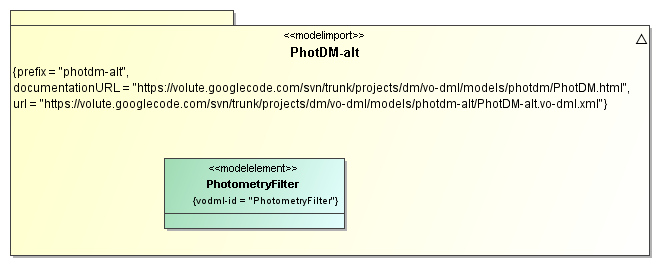
\includegraphics[width=5.51667in,height=2.20833in]{./media/image10.png}

Figure Graphical representation of an imported model. Note the usage of
the stereotype \textless\textless modelimport\textgreater\textgreater{}
and the values assigned to the various tags. Also shown is a type
imported with the model. It must have an explicit vodml-id assigned,
which is accomplished using the
\textless modelelement\textgreater\textgreater{} stereotype (see 4.1 ).

VO-DML/Schema

\textless xsd:complexType name=\emph{"ModelImport"}\textgreater{}

\textless xsd:sequence\textgreater{}

\textless xsd:element name=\emph{"name"} type=\emph{"xsd:string"}
minOccurs=\emph{"1"/}\textgreater{}

\textless xsd:element name=\emph{"identifier"} type=\emph{"xsd:string"}
minOccurs=\emph{"0"/}\textgreater{}

\textless xsd:element name=\emph{"version"} type=\emph{"xsd:string"}
minOccurs=\emph{"1"/}\textgreater{}

\textless xsd:element name=\emph{"url"} type=\emph{"xsd:anyURI"}
\emph{/}\textgreater{}

\textless xsd:element name="documentationURL" type="xsd:anyURI"
/\textgreater{}

\textless/xsd:sequence\textgreater{}

\textless/xsd:complexType\textgreater{}

VO-DML/XML

See 4.4.10.

\hypertarget{name-string-1-1}{%
\subsubsection{name : string {[}1{]}}\label{name-string-1-1}}

Name by which imported model is used in the current model and its
documentation. This name MUST be the same as the 'name' given to the
imported model in the VO-DML document from which it is imported. Each
vodml-ref (4.2.1 ) pointing to an element in the imported model MUST use
this name as prefix.

\hypertarget{identifier-string-0..1}{%
\subsubsection{identifier : string
{[}0..1{]}}\label{identifier-string-0..1}}

The IVOA identifier by which the imported modeled is registered in an
IVOA registry.

\hypertarget{version-string-1-1}{%
\subsubsection{version : string {[}1{]}}\label{version-string-1-1}}

Version of the imported model.

\hypertarget{url-anyuri-1}{%
\subsubsection{url : anyURI {[}1{]}}\label{url-anyuri-1}}

URL from which the imported VO-DML model document can be downloaded.

\hypertarget{documentationurl-anyuri-1}{%
\subsubsection{documentationURL : anyURI
{[}1{]}}\label{documentationurl-anyuri-1}}

URL where a documentation HTML file for the remote model can be
downloaded. This SHOULD be a document that contains anchors for each
element that has as name attribute the vodml-id of that element. I.e. it
is assumed that the vodml-id-s of the imported types can be added onto
this documentationURL as fragments so that a direct link to the
documentation for a referenced data model element can be found.

\hypertarget{type-extends-referableelement}{%
\subsection{\texorpdfstring{\emph{Type} extends
\protect\hyperlink{type-extends-referableelement}{\emph{ReferableElement}}}{Type extends ReferableElement}}\label{type-extends-referableelement}}

The ultimate goal of any VO-DML data model is to describe a part of the
world. The world is assumed to consist of \emph{objects} of some type or
another. Instead of objects one could use the terms \emph{individuals}
(see OWL for example), or \emph{entities} (entity-relationship models).

The most important way the modeling language has for describing this
world of objects is by defining subsets of all these objects. In VO-DML
these subsets are referred to as \textbf{Types}. The Type defines a set
of properties that all objects in the set, also called \emph{instances}
of the Type, possess. VO-DML assumes that every instance in the Universe
of Discourse, i.e. every object "worth talking about" in the context of
the model, must be explicitly assigned to one Type.

\textbf{Type} is abstract and is extended by ultimately four concrete
subtypes.

The most important\footnote{and evidently confusing for non-initiated.}
categorization of \textbf{Types} is that between so called
\textbf{object types} and \textbf{value types}.

An \textbf{object type} represents a full-fledged, possibly very complex
concept in the real world and is built from properties and relations to
other object types. An important feature of object types as opposed to
ValueType-s (see below) is that instances of ObjectTypes, i.e. objects,
have their own, explicit identity\footnote{This is admittedly a somewhat
  theoretical but important object-oriented concept.} that is defined
independent of the state of the object.

A \textbf{value type} represents a simple concept that is generally used
as a building block for defining more complex concepts up to object
types. In contrast to the latter, instances of ValueType-s, i.e.
\emph{values} need not be explicitly identified. They are identified by
their value alone. For example an integer is a value type; all instances
of the integer value '3' represent the same integer. Not all value types
are atomic though, see \textbf{DataType} below.

Another way to express the difference between value types and object
types lies at the heart of why and how databases are built. The
\emph{extent} of a value type, i.e. its set of valid instances/values,
is \emph{self-evident from its definition}. That is, from the definition
one can infer exactly which values exist in the set defined by the value
type. Hence one can identify the instance by its value.

This is not the case for object types. Though one can define a Person
object type with say a name and a date-of-birth for example, one cannot
be sure that any combination of a name and a date will correspond to an
existing person. Moreover, two existing instances named 'Jane' born on
Jan 12 1965 are not by definition the same (instance of) Person. For
object types it is therefore first a meaningful, non-trivial statement
to make that some instance exists, and second to assign an identity to
these instances that is independent of the state of the instance.

And this is precisely what a database does. One will never create a
database and store in it all integers, or all points on the unit sphere,
simply to make the statement that each of these exists. Their existence
is pre-defined by the definition of the sphere.

In contrast, one \emph{does} create databases with information about
persons, possibly containing an integer attribute \emph{age}. Or ones
that store sources observed on the sky, with their position represented
by a point on the sphere and an explicit identifier. Hence sources and
persons are represented by object types integers and
"points-on-the-unit-sphere" by a value type (a PrimitiveType for the
former, a DataType for the latter to be precise).

\protect\hypertarget{_extends:_ElementRef}{}{}

VO-UML

Relevant UML meta-classes:
\href{http://www.uml-diagrams.org/uml-core.html\#type}{\emph{Type}}
{[}§7.3.52{]},
\href{http://www.uml-diagrams.org/classifier.html}{\emph{Classifier}}
{[}§7.3.8{]},
\href{http://www.uml-diagrams.org/generalization.html}{Generalization}
{[}§7.3.20{]}.

\emph{Type} and \emph{Classifier} are abstract meta-classes in UML and
have no graphical representation of their own. \emph{Classifier} extends
\emph{Type} and is itself the super-type of UML meta-classes
\emph{Class} and \emph{DataType} which are represented in VO-DML by
\protect\hyperlink{objecttype-extends-type}{\textbf{ObjectType}} and the
value types
\protect\hyperlink{primitivetype-extends-valuetype}{\textbf{PrimitiveType}},
\protect\hyperlink{enumeration-extends-valuetype}{\textbf{Enumeration}}
and \protect\hyperlink{datatype-extends-valuetype}{\textbf{DataType}}
respectively. All these types are represented graphically by rectangles
with at least the name of the type and possibly the stereotype defining
the particular "type of the type", as shown in Figure 8.

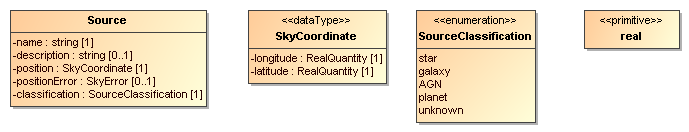
\includegraphics[width=5.74167in,height=1.1in]{./media/image11.png}

Figure Examples of the four different classes of types supported by
VO-DML and their representation. See the definition of the types for
more details.

The inheritance relationship is represented in UML by the
\emph{Generalization} meta-class and graphically by an arrow (always red
in our profile) with a hollow arrow head from sub-type to super-type. In
UML \emph{Generalization} is a special relation between types, in VO-DML
it is simply a pointer (ElementRef) from sub-type to super-type, owned
by the sub-type.

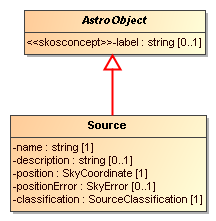
\includegraphics[width=1.8in,height=1.84167in]{./media/image12.png}

VO-DML/Schema

In VO-DML/Schema \textbf{Type} is represented by an abstract complexType
named Type. It is the base-type of all more concrete type definitions.
It extends ReferableElement, hence all type definitions can be
referenced and MUST have a \textless vodml-id\textgreater{} element.
Types may be abstract, in which case no instances can be produced
(similar to for example abstract classes in Java). They may also extend
another type, which will be referred to as the \emph{super-type}. The
super-type is identified by an ElementRef.

\textless xsd:complexType name=\emph{"Type"}
abstract=\emph{"true"}\textgreater{}

\textless xsd:complexContent\textgreater{}

\textless xsd:extension base=\emph{"ReferableElement"}\textgreater{}

\textless xsd:sequence\textgreater{}

\textless xsd:element name=\emph{"extends"} type=\emph{"ElementRef"}
minOccurs=\emph{"0"/}\textgreater{}

\textless xsd:element name=\emph{"constraints"} type=\emph{"Constraint"}

minOccurs=\emph{"0"} maxOccurs=\emph{"unbounded"/}\textgreater{}

\textless/xsd:sequence\textgreater{}

\textless xsd:attribute name=\emph{"abstract"} type=\emph{"xsd:boolean"}

default=\emph{"false"} use=\emph{"optional"} /\textgreater{}

\textless/xsd:extension\textgreater{}

\textless/xsd:complexContent\textgreater{}

\textless/xsd:complexType\textgreater{}

VO-DML/XML

For examples of type definitions see the definitions of the concrete
sub-types of \textbf{Type}. The following snippet is an example of the
extends relationship.

\textless objectType\textgreater{}

\textless vodml-id\textgreater source.Source\textless/vodml-id\textgreater{}

\textless name\textgreater Source\textless/name\textgreater{}

...

\textless extends\textgreater{}

\textless vodml-ref\textgreater src:source.AstroObject\textless/vodml-ref\textgreater{}

\textless/extends\textgreater{}

...

\hypertarget{extends-elementref-0..1}{%
\subsubsection{\texorpdfstring{extends :
\protect\hyperlink{elementref}{ElementRef}
{[}0..1{]}}{extends : ElementRef {[}0..1{]}}}\label{extends-elementref-0..1}}

VO-DML supports the object-oriented concept of inheritance, or
generalization, between \textbf{Types}. Generalization is a directed
binary association between a specialized sub-type and its more general
super-type (the target) identified through the \textbf{extends}
property, which is a reference to the target element.

It defines a sub-set relation between the set of instances defined by
the super-type and that of the sub-type: every instance of a sub-type is
also an instance of the super-type. In contrast to UML, VO-DML does not
support multiple inheritance, i.e. a type can have at most one direct
super-type. Furthermore ObjectTypes can only extend ObjectTypes,
DataTypes can only extend DataTypes etc.

Instances of sub-types inherit all the
\protect\hyperlink{role-extends-referableelement}{\textbf{Roles}} and
\protect\hyperlink{constraint}{\textbf{Constraints}} (see below) defined
on the super-type. This inheritance is applied recursively, i.e. a type
also inherits the roles and constraints its super-type has inherited.

\hypertarget{constraint-constraint-0..}{%
\subsubsection{constraint : Constraint
{[}0..*{]}}\label{constraint-constraint-0..}}

Instances of a \textbf{Type} can be constrained by rules that define
whether they are valid instances. VO-DML allows two types of
constraints: Generic expressions in some computer-readable language,
defined by the \protect\hyperlink{constraint}{\textbf{Constraint}} type
itself, or
\protect\hyperlink{subsettedrole-extends-constraint}{\textbf{SubsettedRole}}-s,
which offers a way to constrain elements of inherited Roles and extends
Constraint.

\hypertarget{valuetype-extends-type}{%
\subsection{\texorpdfstring{\emph{ValueType} extends
\protect\hyperlink{type-extends-referableelement}{\emph{Type}}}{ValueType extends Type}}\label{valuetype-extends-type}}

A \textbf{ValueType} is a special kind of \textbf{Type}, one whose
instances are \emph{values}. See the discussion in the
\protect\hyperlink{type-extends-referableelement}{definition} of
\textbf{Type} for the details on why \textbf{ValueType} is defined.

VO-UML

Nearest UML meta-class:
\href{http://www.uml-diagrams.org/class-diagrams.html\#data-type}{\emph{DataType}}.
{[}§7.3.11{]}

VO-DML has a special concept to represent all value types, whereas UML
uses \emph{DataType} for this. VO-DML defines \textbf{DataType} (see
4.11 ) as a special kind of \textbf{ValueType}.

VO-DML/Schema

\textless xsd:complexType name=\emph{"ValueType"}
abstract=\emph{"true"}\textgreater{}

\textless xsd:complexContent\textgreater{}

\textless xsd:extension base=\emph{"Type"}\textgreater{}

\textless/xsd:extension\textgreater{}

\textless/xsd:complexContent\textgreater{}

\textless/xsd:complexType\textgreater{}

\hypertarget{primitivetype-extends-valuetype}{%
\subsection{\texorpdfstring{PrimitiveType extends
\protect\hyperlink{valuetype-extends-type}{\emph{ValueType}}}{PrimitiveType extends ValueType}}\label{primitivetype-extends-valuetype}}

A PrimitiveType represents an atomic piece of data, a \emph{value} with
no structure. Examples are the standard types like integer, boolean,
real, and string (which is treated as an atomic value, \emph{not} an
array of characters) and so on.

A primitive type can be an extension of another primitive type, but must
then always be considered a restriction on the possible values of that
type. The particular restriction SHOULD be identified using an explicit
Constraint (see 4.20 ) defined on the type.

VO-UML

Derived from UML meta-class:
\href{http://www.uml-diagrams.org/class-diagrams.html\#primitive-type}{\emph{Primitive}
Type} {[}§7.3.44{]}.

A primitive type is represented graphically by an UML DataType, which is
a rectangle containing the name of the type and stereotype
\textless\textless primitive\textgreater\textgreater{} placed above the
name. If it extends an existing type, the Constraint defining the
restriction may be represented by text below the type name as in the
example in the figure.

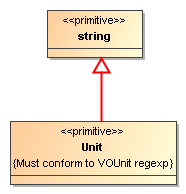
\includegraphics[width=1.55in,height=1.61667in]{./media/image13.png}

VO-DML/SCHEMA

\textless xsd:complexType name=\emph{"PrimitiveType"}\textgreater{}

\textless xsd:complexContent\textgreater{}

\textless xsd:extension base=\emph{"ValueType"}\textgreater{}

\textless/xsd:extension\textgreater{}

\textless/xsd:complexContent\textgreater{}

\textless/xsd:complexType\textgreater{}

VO-DML/XML

\textless primitiveType\textgreater{}

\textless vodml-id\textgreater quantity/Unit\textless/vodml-id\textgreater{}

\textless name\textgreater Unit\textless/name\textgreater{}

\textless description\textgreater{}

Must conform to definition of unit in VOUnit spec.

\textless/description\textgreater{}

\textless extends\textgreater{}

\textless vodml-ref\textgreater ivoa:string\textless/vodml-ref\textgreater{}

\textless/extends\textgreater{}

\textless/primitiveType\textgreater{}

\hypertarget{enumeration-extends-valuetype}{%
\subsection{\texorpdfstring{Enumeration extends
\protect\hyperlink{valuetype-extends-type}{\emph{ValueType}}}{Enumeration extends ValueType}}\label{enumeration-extends-valuetype}}

An Enumeration is a PrimitiveType with a finite list of possible values,
the Literals. This list restricts the domain of possible instances of
the type. Common usage is to identify different categories of a
structured ObjectType or DataType that uses the Enumeration as an
Attribute. The literals are meant to identify these distinct categories.

Care should be taken in defining Enumerations and Attributes using them.
In particular a choice must be made between introducing such a new type
in the model and assigning a semantic vocabulary to the attribute (see
4.14.1 ). In particular if the set of concepts or categories might
change over time it is better to use the latter approach.

An important consideration is whether the definition of the type defines
automatically all its instances, the characteristic of a ValueType..

\protect\hypertarget{_Literal}{}{}VO-UML

Essentially equivalent to UML meta-class
\href{http://www.uml-diagrams.org/class-diagrams.html\#enumeration}{\emph{Enumeration}}
{[}§7.3.16{]}

An enumeration is represented graphically by the element for a UML
DataType with the stereotype
\textless\textless enumeration\textgreater\textgreater{} above the name
of the type. Below the name the literals are listed.

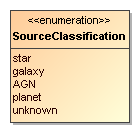
\includegraphics[width=1.15833in,height=1.1in]{./media/image14.png}

Figure Example enumeration listing a number of literals representing
source classifications.

VO-DML/XSD

\textless xsd:complexType name=\emph{"Enumeration"}\textgreater{}

\textless xsd:complexContent\textgreater{}

\textless xsd:extension base=\emph{"PrimitiveType"}\textgreater{}

\textless xsd:sequence\textgreater{}

\textless xsd:element name=\emph{"literal"} type=\emph{"EnumLiteral"}

maxOccurs=\emph{"unbounded"}\textgreater{}

\textless/xsd:element\textgreater{}

\textless/xsd:sequence\textgreater{}

\textless/xsd:extension\textgreater{}

\textless/xsd:complexContent\textgreater{}

\textless/xsd:complexType\textgreater{}

VO-DML/XML

\textless enumeration\textgreater{}

\textless vodml-id\textgreater source.SourceClassification\textless/vodml-id\textgreater{}

\textless name\textgreater SourceClassification\textless/name\textgreater{}

\textless literal\textgreater{}

\textless vodml-id\textgreater source.SourceClassification.star\textless/vodml-id\textgreater{}

\textless name\textgreater star\textless/name\textgreater{}

\textless description\textgreater...\textless/description\textgreater{}

\textless/literal\textgreater{}

\textless literal\textgreater{}

\textless vodml-id\textgreater source.SourceClassification.galaxy\textless/vodml-id\textgreater{}

\textless name\textgreater galaxy\textless/name\textgreater{}

\textless description\textgreater...\textless/description\textgreater{}

\textless/literal\textgreater{}

...

\hypertarget{literal-enumliteral-1..}{%
\subsubsection{\texorpdfstring{literal :
\protect\hyperlink{enumliteral-extends-referableelement}{EnumLiteral}
{[}1..*{]}}{literal : EnumLiteral {[}1..*{]}}}\label{literal-enumliteral-1..}}

An \textbf{Enumeration} is defined by a collection of
\textbf{literal}-s, basically just names with a vodml-id and a
description. The literals are modeled as strings, as the actual value of
an enumeration literal is not important, only its meaning and the fact
that the values must be distinct. Similar to the interpretation of the
inheritance relationship of \textbf{PrimitiveTypes}, a sub-type of an
\textbf{Enumeration} must restrict the set of accessible values and
should explicitly define the literals it allows among the literals
defined by the super-type.

\hypertarget{enumliteral-extends-referableelement}{%
\subsection{\texorpdfstring{EnumLiteral extends
\protect\hyperlink{referableelement}{\emph{ReferableElement}}}{EnumLiteral extends ReferableElement}}\label{enumliteral-extends-referableelement}}

\textbf{EnumLiteral} does not add any new features to
\textbf{ReferableElement}. Note that the literal's value is defined by
the \textbf{name} attribute inherited from ReferableElement. A literal
\emph{is-a} ReferableElement because we may want to refer to it. The
main use case for this is where an existing data(base) model for example
has its own list of values which are not identical to the values used in
the Enumeration. An explicit mapping to the enumeration literals allows
one to make the required translation.

Because of its likely use in defining the vodml-id, the literal has the
same restrictions defined by the VODMLNAME pattern.

VO-UML

\textbf{EnumLiteral} is equivalent to UML meta-class
\emph{EnumerationLiteral} {[}§7.3.17{]}

VO-DML/XSD

\textless xsd:complexType name=\emph{"EnumLiteral"}\textgreater{}

\textless xsd:complexContent\textgreater{}

\textless xsd:extension base=\emph{"ReferableElement"}\textgreater{}

\textless xsd:sequence\textgreater{}

\textless/xsd:sequence\textgreater{}

\textless/xsd:extension\textgreater{}

\textless/xsd:complexContent\textgreater{}

\textless/xsd:complexType\textgreater{}

\hypertarget{datatype-extends-valuetype}{%
\subsection{\texorpdfstring{DataType extends
\protect\hyperlink{valuetype-extends-type}{\emph{ValueType}}}{DataType extends ValueType}}\label{datatype-extends-valuetype}}

A \textbf{DataType} is a value type with structure. The structure is
generally defined by \textbf{attributes} on the \textbf{DataType}, and
possibly \textbf{references}. The state of instance of a DataType, i.e.
a \emph{value}, consists of the assignment of values to all the
attributes and references. This is similar to \textbf{ObjectTypes}
defined below, but in contrast to \textbf{ObjectTypes},
\textbf{DataTypes} have \emph{no} explicit identity. As is the case for
the other \textbf{ValueTypes}, \textbf{DataTypes} are defined by their
state only. I.e. two \textbf{DataType} instances with the same state are
the same instance. Instead, \textbf{ObjectTypes} with the same state but
different identity are not the same

For example the \textbf{DataType} Position3D, with attributes x, y, and
z, is completely defined by the values of the three attributes.
Logically, there are no 2 distinct instances of this \textbf{DataType}
with exact same values (x=1.2, y=2.3, z=3.4). Note, however, that this
statement does not have implications on the implementations: one might
indeed have two instances of a \textbf{DataType} at two distinct memory
locations with the same state. However, an equality test on those
concrete instances should always return `true' as long as they have the
same state.

Also, this specification does not provide any requirements regarding the
immutability of \textbf{DataType} instances, i.e. whether or not it is
possible to change one value of a \textbf{DataType} instance without
requiring a new concrete instance to be created from scratch. As far as
the VO-DML meta-model is concerned, two \textbf{DataType} instances with
different states are always, logically, distinct instances. However, we
do not specify how such behavior has to be interpreted in
implementations. As \textbf{DataType}s can, in principle, be arbitrarily
complex in structure, an implementation might make their instances
mutable for the sake of simplicity.

\textbf{DataType} can have outgoing \textbf{references} with target an
\textbf{ObjectType}. This makes certain patterns more reusable. The
\textbf{reference} is assumed to provide reference data with respect to
which the rest of the value should be interpreted. For example
SkyCoordinate may have a \textbf{reference} to a SkyCoordinateFrame to
help interpret the values of the longitude/latitude \textbf{attributes}.

VO-UML

Derived from UML meta-class:
\href{http://www.uml-diagrams.org/class-diagrams.html\#data-type}{Data
Type} {[}§7.3.11{]}

This concept is represented graphically by a box with stereotype
\textless\textless dataType\textgreater\textgreater{} and possibly
attributes and reference relations.

Note that VO-UML enforces a specific notation for attributes that are
\textbf{DataType}s or \textbf{ObjectType}s, whereas UML allows some
freedom of notation. In particular, attributes that are
\textbf{DataType}s should always be included in the box representing the
owning type, while attributes that are \textbf{ObjectType}s should
always be represented as distinct boxes made targets of an association.

As VO-UML is not normative, alternative graphical representations are
fine as long as they conform to UML rules and that they are explicitly
noted.

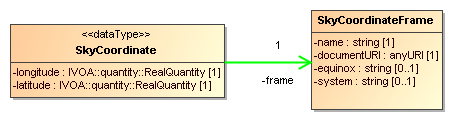
\includegraphics[width=3.76667in,height=0.99167in]{./media/image15.png}

Figure DataType SkyCoordinate is defined as a longitude/latitude pair
with a reference to a reference frame that allows the interpretation of
the values of the attributes.

VO-UML/Schema

\textless xsd:complexType name=\emph{"DataType"}\textgreater{}

\textless xsd:complexContent\textgreater{}

\textless xsd:extension base=\emph{"ValueType"}\textgreater{}

\textless xsd:sequence\textgreater{}

\textless xsd:element name=\emph{"attribute"} type=\emph{"Attribute"}

minOccurs=\emph{"0"} maxOccurs=\emph{"unbounded"/}\textgreater{}

\textless xsd:element name=\emph{"reference"} type=\emph{"Reference"}

minOccurs=\emph{"0"} maxOccurs=\emph{"unbounded"/}\textgreater{}

\textless/xsd:sequence\textgreater{}

\textless/xsd:extension\textgreater{}

\textless/xsd:complexContent\textgreater{}

\textless/xsd:complexType\textgreater{}

VO-UML/XML

\textless dataType\textgreater{}

\textless vodml-id\textgreater source.SkyCoordinate\textless/vodml-id\textgreater{}

\textless name\textgreater SkyCoordinate\textless/name\textgreater{}

\textless description\textgreater...\textless/description\textgreater{}

\textless attribute\textgreater{}

\textless vodml-id\textgreater source.SkyCoordinate.longitude\textless/vodml-id\textgreater{}

\textless name\textgreater longitude\textless/name\textgreater{}

\textless description\textgreater...\textless/description\textgreater{}

\textless datatype\textgreater{}

\textless vodml-ref\textgreater ivoa:quantity.RealQuantity\textless/vodml-ref\textgreater{}

\textless/datatype\textgreater{}

\textless multiplicity\textgreater1\textless/multiplicity\textgreater{}

\textless/attribute\textgreater{}

\textless attribute\textgreater{}

\textless vodml-id\textgreater source.SkyCoordinate.latitude\textless/vodml-id\textgreater{}

\textless name\textgreater latitude\textless/name\textgreater{}

\textless description\textgreater...\textless/description\textgreater{}

\textless datatype\textgreater{}

\textless vodml-ref\textgreater ivoa:quantity.RealQuantity\textless/vodml-ref\textgreater{}

\textless/datatype\textgreater{}

\textless multiplicity\textgreater1\textless/multiplicity\textgreater{}

\textless/attribute\textgreater{}

\textless reference\textgreater{}

\textless vodml-id\textgreater source.SkyCoordinate.frame\textless/vodml-id\textgreater{}

\textless name\textgreater frame\textless/name\textgreater{}

\textless description\textgreater...\textless/description\textgreater{}

\textless datatype\textgreater{}

\textless vodml-ref\textgreater src:source.SkyCoordinateFrame\textless/vodml-ref\textgreater{}

\textless/datatype\textgreater{}

\textless multiplicity\textgreater1\textless/multiplicity\textgreater{}

\textless/reference\textgreater{}

\textless/dataType\textgreater{}

\hypertarget{attribute-attribute-0..}{%
\subsubsection{\texorpdfstring{attribute:
\protect\hyperlink{attribute-extends-role}{Attribute}
{[}0..*{]}}{attribute: Attribute {[}0..*{]}}}\label{attribute-attribute-0..}}

\textbf{Attributes} are structural features of \textbf{DataTypes} and
also \textbf{ObjectTypes}. They represent the role a \textbf{ValueType}
plays in the definition of the parent type. They are like columns in a
table, simple elements in XML etc., though of course the Attribute might
itself be a structured \textbf{DataType}.

\hypertarget{reference-reference-0..}{%
\subsubsection{\texorpdfstring{reference:
\protect\hyperlink{reference-extends-relation}{Reference}
{[}0..*{]}}{reference: Reference {[}0..*{]}}}\label{reference-reference-0..}}

\textbf{References} represent the role an ObjectType plays in the value
of a structured type. A \textbf{reference} on a DataType is assumed to
provide reference data to help interpreting the values of the attributes
of the type. For example a \textbf{DataType} representing a "position on
the sky" needs a \textbf{reference} to a reference frame to ensure that
its \textbf{attributes} longitude and latitude are interpreted properly.

\hypertarget{objecttype-extends-type}{%
\subsection{\texorpdfstring{ObjectType extends
\protect\hyperlink{type-extends-referableelement}{\emph{Type}}}{ObjectType extends Type}}\label{objecttype-extends-type}}

As described in the section of
\protect\hyperlink{type-extends-referableelement}{\textbf{Type}} next to
\textbf{value types,} the other major group of types are \textbf{object
types}. To make this explicit their representation in VO-DML is named
\textbf{ObjectType\emph{.}} They are the fundamental building blocks of
almost every data model, are in fact the reason most data models get
built especially if they aim to serve as the model (schema) of some
database. A database is basically a collection of those objects for
which it is meaningful to store special information. Though generally
ignored, the first important statement made of these database objects is
actually simply that they exist, second that they have certain
properties. \textbf{ObjectType} is meant for representing such kind of
data model elements. Those for which their existence is \emph{not
self-evident} from the definition of the Type they belong to.

VO-UML

Derived from UML meta-class
\href{http://www.uml-diagrams.org/class-diagrams.html\#class}{\emph{Class}}
{[}§7.3.7{]}.

VO-DML does not follow UML's use of the name \emph{Class}, as the phrase
is too commonly used in many of the possible serialization contexts.
E.g. most if not all object oriented languages use "class" for all
structured types. SmallTalk even uses it for all types.

VO-UML represents \textbf{ObjectType} graphically by a rectangle with a
name and possibly a custom \emph{stereotype} such as
\textless\textless modelelement\textgreater\textgreater. An
\textbf{ObjectType} may have attributes and be the source or target of
relationships.

Note that VO-UML enforces a specific notation for attributes that are
\textbf{DataType}s or \textbf{ObjectType}s, whereas UML allows some
freedom of notation. In particular, attributes that are
\textbf{DataType}s should always be included in the box representing the
owning type, while attributes that are \textbf{ObjectType}s should
always be represented as distinct boxes made targets of a named
association.

As VO-UML is not normative, alternative graphical representations are
fine as long as they conform to UML rules and they are explicitly mapped
to the VO-UML notation.

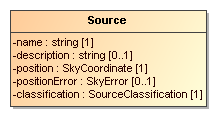
\includegraphics[width=1.8in,height=0.96667in]{./media/image16.png}

VO-DML/Schema

In XSD the \textbf{ObjectType} is represented by a complexType
definition ObjectType that extends Type.

\textless xsd:complexType name=\emph{"ObjectType"}\textgreater{}

\textless xsd:complexContent\textgreater{}

\textless xsd:extension base=\emph{"Type"}\textgreater{}

\textless xsd:sequence\textgreater{}

\textless xsd:element name=\emph{"attribute"} type=\emph{"Attribute"}

minOccurs=\emph{"0"} maxOccurs=\emph{"unbounded"/}\textgreater{}

\textless xsd:element name=\emph{"composition"}
type=\emph{"Composition"}

minOccurs=\emph{"0"} maxOccurs=\emph{"unbounded"/}\textgreater{}

\textless xsd:element name=\emph{"reference"} type=\emph{"Reference"}

minOccurs=\emph{"0"} maxOccurs=\emph{"unbounded"/}\textgreater{}

\textless/xsd:sequence\textgreater{}

\textless/xsd:extension\textgreater{}

\textless/xsd:complexContent\textgreater{}

\textless/xsd:complexType\textgreater{}

VO-DML/XML

\textless objectType\textgreater{}

\textless vodml-id\textgreater source.Source\textless/vodml-id\textgreater{}

\textless name\textgreater Source\textless/name\textgreater{}

\textless description\textgreater...\textless/description\textgreater{}

\textless extends\textgreater{}

\textless vodml-ref\textgreater src:source.AstroObject\textless/vodml-ref\textgreater{}

\textless/extends\textgreater{}

...

\textless/objcectType\textgreater{}

\hypertarget{attribute-attribute-0..-1}{%
\subsubsection{\texorpdfstring{attribute :
\protect\hyperlink{attribute-extends-role}{Attribute}
{[}0..*{]}}{attribute : Attribute {[}0..*{]}}}\label{attribute-attribute-0..-1}}

Collection of Attribute definitions.

\hypertarget{composition-composition-0..}{%
\subsubsection{\texorpdfstring{composition :
\protect\hyperlink{composition-extends-relation}{Composition}
{[}0..*{]}}{composition : Composition {[}0..*{]}}}\label{composition-composition-0..}}

Collection of \textbf{Composition} relations owned by the object type.
This relation between \textbf{ObjectTypes} indicates that an instance of
the owner of the composition, the \emph{parent}, is \emph{composed of}
other objects, sometimes referred to as \emph{children}. This is a very
strong ``has-a'' relationship. It indicates for example that (in the
model) an instance of the child object type cannot exist without an
instance of the parent\footnote{This does \emph{not} mean that one
  cannot have serialized representations of child objects without their
  parent. This purely depends on the serialization format and possibly
  the query producing the result.}. Also, a child object cannot be
swapped between parents during the life cycle of those. And finally a
certain \textbf{ObjectType} can only be \emph{contained in} one parent
\textbf{ObjectType}. And the counting includes potential containment
relations inherited through a super-type. I.e. if \textbf{ObjectType} A
has a composition of B-s, any sub-type of B is bound by this relation.
And \emph{no} sub-type of B can be the child in a containment
relationship.

These constraints enforce models that are consistent and that can be
easily represented in many different contexts, ranging from database
management systems to object oriented applications. It is easy to find
solutions that work around these constraints if one really needs to, but
in general such constraints are useful to help modelers avoiding
modeling solutions that would prove to be problematic from the
interoperability point of view.

Note that implementations of the \textbf{Composition} relationship
usually provide means to navigate from the contained instance to its
container. However, this is left out of this specification and freedom
is left to the implementations to provide such mechanisms. This is also
true for serialization strategies, which should always allow clients to
navigate from the contained instances to their containers.

\hypertarget{reference-reference-0..-1}{%
\subsubsection{\texorpdfstring{reference:
\protect\hyperlink{reference-extends-relation}{Reference}
{[}0..*{]}}{reference: Reference {[}0..*{]}}}\label{reference-reference-0..-1}}

Collection of \textbf{Reference} definitions. The reference relation is
the second type of relation between \textbf{ObjectType}s. It is a much
looser relation than composition. The interpretation is here more
general than the one for the reference collection on \textbf{DataType}.
Relations here can have meaning beyond providing reference data for
interpreting the attributes.

It is important to note that in a \textbf{Reference} relation the life
cycles of both ends of the relation itself are completely independent.
This also means that there is, in general, no way for clients to
navigate from the referenced instance to the instances that reference
them, unless the specific implementations provide such mechanisms
according to their requirements.

\hypertarget{role-extends-referableelement}{%
\subsection{\texorpdfstring{\emph{Role} extends
\protect\hyperlink{type-extends-referableelement}{\emph{ReferableElement}}}{Role extends ReferableElement}}\label{role-extends-referableelement}}

A \textbf{Role} represents the usage of one type (call it "target") in
the definition of another (call it "source"). The "target" type is said
to play a role in the definition of the "source" type. Examples are
where the target is the super-type of the source, or where the target is
the data type of an attribute defined on the source.

There are different kinds of roles, in VO-DML defined as sub-types of
\emph{Role}. \emph{Role} defines only a "data type" attribute that has
an ElementRef as data type, but is constrained by Schematron rules to
reference a Type. Specializations of Role will introduce further
constraints.

VO-UML

\textbf{Role} is similar to the UML concepts
\href{http://www.uml-diagrams.org/uml-core.html\#feature}{\emph{Feature}}
{[}§7.3.19{]},
\href{http://www.uml-diagrams.org/uml-core.html\#structural-feature}{\emph{StructuralFeature}}
{[}§7.3.50{]},
\href{http://www.uml-diagrams.org/uml-core.html\#type}{\emph{TypedElement}}
{[}§7.3.53{]} and
\href{http://www.uml-diagrams.org/property.html}{\emph{Property}}
{[}§7.3.45{]}. The sub-types of \textbf{Role} make this correspondence
more concrete.

VO-DML/Schema

\textbf{Role} is explicitly represented in the VO-DML/Schema. It
contains child elements \textbf{datatype} that identifies (through a
\textless vodml-ref\textgreater) the type that is playing the role on
the parent type containing the role, and \textbf{multiplicity} that
defines the cardinality of the attribute, i.e. how many instances of the
data type can be added to the parent type. \textbf{Role} is abstract,
hence only subclasses can be instantiated. The subclasses define more
restrictions on the datatype and multiplicity attributes.

\textless xsd:complexType name=\emph{"Role"}
abstract=\emph{"true"}\textgreater{}

\textless xsd:complexContent\textgreater{}

\textless xsd:extension base=\emph{"ReferableElement"}\textgreater{}

\textless xsd:sequence\textgreater{}

\textless xsd:element name=\emph{"datatype"} type=\emph{"ElementRef"
minOccurs="1"/}\textgreater{}

\textless xsd:element name=\emph{"multiplicity"}
type=\emph{"Multiplicity"}

\emph{minOccurs="0"/}\textgreater{}

\textless/xsd:sequence\textgreater{}

\textless/xsd:extension\textgreater{}

\textless/xsd:complexContent\textgreater{}

\textless/xsd:complexType\textgreater{}

\hypertarget{datatype-elementref}{%
\subsubsection{\texorpdfstring{datatype :
\protect\hyperlink{elementref}{ElementRef}}{datatype : ElementRef}}\label{datatype-elementref}}

The \textbf{datatype} property of a Role identifies the target type of
the role, the one that actually "plays the role". In VO-DML/Schema it is
represented by an ElementRef that MUST identify a Type.

\hypertarget{multiplicity-multiplicity}{%
\subsubsection{\texorpdfstring{multiplicity:
\protect\hyperlink{multiplicity}{Multiplicity}}{multiplicity: Multiplicity}}\label{multiplicity-multiplicity}}

Indicates the multiplicity or cardinality of the role. This indicates
how many instances of the target \textbf{datatype} can be assigned to
the role property.

\hypertarget{attribute-extends-role}{%
\subsection{\texorpdfstring{Attribute extends
\protect\hyperlink{role-extends-referableelement}{\emph{Role}}}{Attribute extends Role}}\label{attribute-extends-role}}

An \textbf{Attribute} is the role that a \textbf{ValueType} can play in
the definition of a structured type, i.e. an \textbf{ObjectType} or
\textbf{DataType}. It represents a typical property of the parent type
such as age, mass, length, position etc.

\textbf{Attribute} restricts the possible types of the \textbf{Role}'s
datatype attribute to \textbf{ValueType}-s only. Please refer to the
definition of the
\protect\hyperlink{multiplicity}{\textbf{Multiplicity}} type for some
special restrictions and interpretations on Attribute multiplicities.

VO-UML

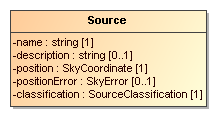
\includegraphics[width=1.8in,height=0.96667in]{./media/image16.png}

Figure . The rows in the lower part of the box represent attributes.
Their name, datatype and multiplicity are indicated.

VO-DML/Schema

\textless xsd:complexType name=\emph{"Attribute"}\textgreater{}

\textless xsd:complexContent\textgreater{}

\textless xsd:extension base=\emph{"Role"}\textgreater{}

\textless xsd:sequence\textgreater{}

\textless xsd:element name=\emph{"semanticconcept"}
type=\emph{"SemanticConcept"}

minOccurs=\emph{"0"/}\textgreater{}

\textless/xsd:sequence\textgreater{}

\textless/xsd:extension\textgreater{}

\textless/xsd:complexContent\textgreater{}

\textless/xsd:complexType\textgreater{}

VO-DML/XML

\textless objectType\textgreater{}

\textless vodml-id\textgreater source.Source\textless/vodml-id\textgreater{}

\textless name\textgreater Source\textless/name\textgreater{}

...

\textless attribute\textgreater{}

\textless vodml-id\textgreater source.Source.name\textless/vodml-id\textgreater{}

\textless name\textgreater name\textless/name\textgreater{}

\textless description\textgreater...\textless/description\textgreater{}

\textless datatype\textgreater{}

\textless vodml-ref\textgreater ivoa:string\textless/vodml-ref\textgreater{}

\textless/datatype\textgreater{}

\textless multiplicity\textgreater{}

\textless minOccurs\textgreater1\textless/minOccurs\textgreater{}

\textless maxOccurs\textgreater1\textless/maxOccurs\textgreater{}

\textless/multiplicity\textgreater{}

\textless/attribute\textgreater{}

...

\hypertarget{semanticconcept-semanticconcept-0..1}{%
\subsubsection{\texorpdfstring{semanticconcept :
\protect\hyperlink{semanticconcept}{SemanticConcept}
{[}0..1{]}}{semanticconcept : SemanticConcept {[}0..1{]}}}\label{semanticconcept-semanticconcept-0..1}}

If an Attribute definition contains a \textbf{semanticconcept} it
implies the value of the attribute should be able to identify a concept
in some semantic vocabulary. This may be a SKOS vocabulary as in
{[}17{]}, but it may be more general, see the definition of the
\protect\hyperlink{semanticconcept}{SemanticConcept} definition. In this
case the data type attribute should be compatible with a string.

\hypertarget{semanticconcept}{%
\subsection{SemanticConcept}\label{semanticconcept}}

It is a common pattern in data modeling that one wishes to constrain the
set of values on an attribute to some predefined list. One way to do so
is using an
\protect\hyperlink{enumeration-extends-valuetype}{Enumeration} as the
attribute's \protect\hyperlink{datatype-elementref}{datatype}. A user of
a data model knows immediately that the elements of the enumeration are
exhaustive and exclusive, and also that they are reasonably slow to
change. These features can sometimes, however, be disadvantages, for
example when a list of terms might be very large and should be allowed
to evolve over time, or is predefined and possibly maintained by another
party.~ In such cases, the values should be constrained by some external
semantic structure, references to which are supported by the
\textbf{SemanticConcept} type.

This mechanism should not be taken as an invitation to subvert the main
VO-DML model by introducing arbitrary external modelling frameworks.~
The two mechanisms described below, using SKOS vocabularies and RDFS
sub-classing, are intended to be illustrative rather than exhaustive,
and if these are felt to be insufficient for some reason, the
alternative should be compatible in spirit with these.

SKOS vocabularies: The IVOA Recommendation \emph{Vocabularies in the
Virtual Observatory} specifies that the format for such vocabularies
should be "based on the W3C's Resource Description Framework (RDF) and
the Simple Knowledge Organization System (SKOS)" {[}17{]}.~ When using a
SKOS vocabulary as the external semantic structure, the
\textbf{topconcept} attribute names a SKOS Concept (that is, an instance
of skos:Concept): all of the actual values of the associated attribute
must be narrower than this Concept.~ To be precise, for a top concept T,
any concept c is a valid value for this property, if either:

~~ c skos:broaderTransitive T .

or if there exists a concept X such that

~~ c skos:broaderTransitive X. X skos:broadMatch T.

(this just means that, if c is in the same vocabulary as T, then it's
connected by a chain of any number of skos:broader, and if it's in a
different vocabulary, then there is some X which is in the same
vocabulary as c, with a cross-vocabulary link between X and T).

The SKOS thesaurus-based approach is most useful in the context of
searching and browsing of resources.~ It is not intended to be useful
for any sort of inferencing, and in particular does not support a
subclassing or 'Is-A' relationship.~ Although it might be tempting to
say, for example, something like 'calibration-image' skos:narrower
'dark-image', one is not formally permitted to conclude from this that a
dark is a type of calibration image (even though that is true).\\
\strut \\
RDFS ontologies: The RDF Schema standard
\textless{}\url{http://www.w3.org/TR/rdf-schema/}\textgreater{} provides
the minimal structures which are necessary for simple ontologies, and
the inferencing associated with them.~ It includes domain and range
constraints, and subtyping of classes and properties, but cannot, for
example, express exclusivity of two terms.~ If the external semantic
structure is of this type, then the topconcept attribute names an
rdfs:Class (not an rdfs:Property), and the actual instances of the
associated attribute must be (transitively) rdfs:subClassOf this class.

It is not necessary to indicate in the VO-DML model which of these
options has been chosen, since the URI which is the value of the
attribute will contain its own typing information.

VO-UML

\textbf{SemanticConcept} has no explicit representation in UML.

In VO-UML one may represent it using a stereotype
\textless\textless semanticconcept\textgreater\textgreater{} that can be
assigned to attributes. The stereotype can be given tag definitions for
the vocabularyURI and the topConcept attributes as in the MagicDraw
example in Figure 12.

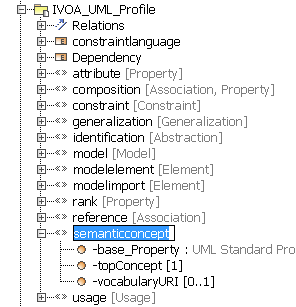
\includegraphics[width=2.46688in,height=2.55856in]{./media/image17.png}

Figure Definition of a
\textless\textless semanticconcept\textgreater\textgreater{} stereotype
with tag definitions for topConcept and vocabularyURI.

This can now be assigned to an attribute as in the example in Figure 13

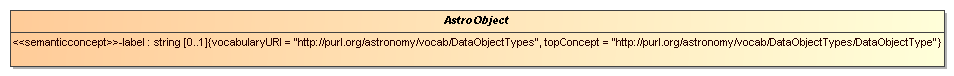
\includegraphics[width=7.96667in,height=0.86875in]{./media/image18.png}

Figure Assignment of
\textless\textless semanticconcept\textgreater\textgreater{} stereotype
to the attribute \emph{label} in the object type \emph{AstroObject}.
Here the vocabularyURI identifies a vocabulary of astronomical object
types.

VO-DML/Schema

\textless xsd:complexType name=\emph{"SemanticConcept"}\textgreater{}

\textless xsd:sequence\textgreater{}

\textless xsd:element name=\emph{"topConcept"} type=\emph{"xsd:anyURI"}

minOccurs=\emph{"0"}\textgreater{}

\textless/xsd:element\textgreater{}

\textless xsd:element name=\emph{"vocabularyURI"}
type=\emph{"xsd:anyURI"} minOccurs=\emph{"0"}

maxOccurs=\emph{"unbounded"}\textgreater{}

\textless/xsd:element\textgreater{}

\textless/xsd:sequence\textgreater{}

\textless/xsd:complexType\textgreater{}

VO-DML/XML

\textless objectType abstract=\emph{"true"}\textgreater{}

\textless vodml-id\textgreater source.AstroObject\textless/vodml-id\textgreater{}

\textless name\textgreater AstroObject\textless/name\textgreater{}

\textless attribute\textgreater{}

\textless vodml-id\textgreater source.AstroObject.label\textless/vodml-id\textgreater{}

\textless name\textgreater label\textless/name\textgreater{}

\textless description\textgreater{}

...

\textless/description\textgreater{}

\textless datatype\textgreater{}

\textless vodml-ref\textgreater ivoa:string\textless/vodml-ref\textgreater{}

\textless/datatype\textgreater{}

\textless multiplicity\textgreater{}

\textless minOccurs\textgreater0\textless/minOccurs\textgreater{}

\textless maxOccurs\textgreater1\textless/maxOccurs\textgreater{}

\textless/multiplicity\textgreater{}

\textless semanticconcept\textgreater{}

\textless topConcept\textgreater{}

\url{http://purl.org/astronomy/vocab/DataObjectTypes/DataObjectType}

\textless/topConcept\textgreater{}

\textless vocabularyURI\textgreater{}

\url{http://purl.org/astronomy/vocab/DataObjectTypes}

\textless/vocabularyURI\textgreater{}

\textless/semanticconcept\textgreater{}

\textless/attribute\textgreater{}

\textless/objectType\textgreater{}

\hypertarget{vocabularyuri-anyuri-0..1}{%
\subsubsection{vocabularyURI: anyURI
{[}0..1{]}}\label{vocabularyuri-anyuri-0..1}}

If this attribute is given a value, it indicates that the attribute to
which the SemanticConcept has been assigned MUST take values from the
vocabulary identified by the URI. It may be possible to define a subset
of its values using the topConcept attribute.

\hypertarget{topconcept-anyuri-0..1}{%
\subsubsection{topConcept: anyURI
{[}0..1{]}}\label{topconcept-anyuri-0..1}}

If this attribute is set, the specified URI identifies a semantic
concept and the value of the Attribute to which the
\textbf{SemanticConcept} has been assigned must themselves be semantic
concepts that are narrower than this broadest concept in the sense
described above. If also the vocabularyURI is set, the values of the
Attribute must come from the vocabulary identified by that URI as well.

\hypertarget{relation-extends-role}{%
\subsection{\texorpdfstring{\emph{Relation} extends
\protect\hyperlink{role-extends-referableelement}{\emph{Role}}
}{Relation extends Role }}\label{relation-extends-role}}

A \textbf{Relation} is a \textbf{Role} played by a (target)
\textbf{ObjectType} in the definition of a (source) \textbf{ObjectType}
or \textbf{DataType}. It indicates that the target of the relation is
related in some fashion to the source type. It also implies a relation
between instances of the target and the source. For this reason the
\textbf{Generalization} construct is \emph{not} a \textbf{Relation}.

VO-DML defines two concrete refinements of Relation,
\protect\hyperlink{composition-extends-relation}{\textbf{Composition}}
and \protect\hyperlink{reference-extends-relation}{\textbf{Reference}}
that embody the different semantics of composite and shared
relationships. The precise details of a particular \textbf{Relation}
defined in a model must be described using its \textbf{description}
attribute.

VO-UML

\textbf{Relation} is a combination of UML's
\href{http://www.uml-diagrams.org/association.html}{Association} and
\href{http://www.uml-diagrams.org/association.html\#association-end}{Association
End} elements:

Whereas in UML associations are first class elements that are directly
owned by a package or model, in VO-DML it is always the source
\textbf{ObjectType} that defines and owns the \textbf{Relation}. This is
equivalent to constraining each UML association to always have a
navigable association end.

In VO-UML \textbf{Relations} are indicated by arrows from the source to
the target in the relation with a \textbf{name} and
\textbf{multiplicity} written near the target. Details depend on the
type of relation.

VO-XML/Schema

\textless xsd:complexType name=\emph{"Relation"}
abstract=\emph{"true"}\textgreater{}

\textless xsd:annotation\textgreater{}

\textless xsd:documentation\textgreater{}

A relation is a Role where the target datatype is an ObjectType.

\textless/xsd:documentation\textgreater{}

\textless/xsd:annotation\textgreater{}

\textless xsd:complexContent\textgreater{}

\textless xsd:extension base=\emph{"Role"}\textgreater{}

\textless xsd:sequence\textgreater{}

\textless/xsd:sequence\textgreater{}

\textless/xsd:extension\textgreater{}

\textless/xsd:complexContent\textgreater{}

\textless/xsd:complexType\textgreater{}

\hypertarget{composition-extends-relation}{%
\subsection{\texorpdfstring{Composition extends
\protect\hyperlink{relation-extends-role}{\emph{Relation}}}{Composition extends Relation}}\label{composition-extends-relation}}

\textbf{Composition} is a special type of \textbf{Relation} that
represents the fact that often an object can be seen to be "composed of"
other objects. This is often called a \emph{whole-parts} relationship.
We will also refer to it as a parent-child relation\footnote{One may
  also say the parent has a \emph{collection} of the child type, or that
  the parent \emph{contains} the child type.}. Examples are the
relationship between an image and the pixels it is composed of, or a bit
more abstractly, a source catalogue and its sources.

This is quite a strong relationship, stronger than the
\protect\hyperlink{reference-extends-relation}{\textbf{Reference}}
relation discussed later. For example the life cycles of the child
objects are governed by that of the parent. When an image is destroyed,
so are its pixels; when a source catalogue is discarded so are its
sources. Similarly an object can only be a part of a single parent, i.e.
the relation is \emph{not} shared.

At the modeling level it is almost invariably true that the part/child
types are defined as a result of an analysis of the parent type. I.e.
their definitions are generally tightly bound. VO-DML formalizes this by
adding the constraint that an \textbf{ObjectType} can only be the target
of at most one \textbf{Composition} relation. The counting should
include relationships inherited from a super-type, i.e. if a super-type
is already contained in a parent, then none of its sub-types may be
declared to be contained. This constraint facilitates the analysis of
models as well as for example the mapping to the relational
model\footnote{In the relational model a composition relation is
  generally represented by a foreign key form the table representing the
  child to the table representing the parent. See also Appendix B.2.}.

VO-UML

In VO-UML a composition relation is represented by a composition
association, an arrow with a filled, closed diamond indicating a
composition side of the container and an arrow on the end of the
contained class. In the UML Profile used for the diagrams a blue color
is used for this relation

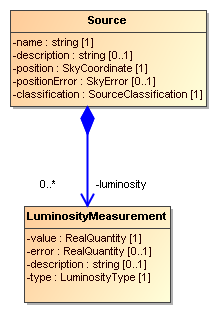
\includegraphics[width=1.8in,height=2.6in]{./media/image19.png}

Figure Composition Relation between two object types.

VO-DML/Schema

\textless xsd:complexType name=\emph{"Composition"}\textgreater{}

\textless xsd:complexContent\textgreater{}

\textless xsd:extension base=\emph{"Relation"}\textgreater{}

\textless xsd:sequence\textgreater{}

\textless xsd:element name=\emph{"isOrdered"} type=\emph{"xsd:boolean"}

default=\emph{"false"} minOccurs=\emph{"0"}\textgreater{}

\textless/xsd:element\textgreater{}

\textless/xsd:sequence\textgreater{}

\textless/xsd:extension\textgreater{}

\textless/xsd:complexContent\textgreater{}

\textless/xsd:complexType\textgreater{}

VO-DML/XML

\textless objectType\textgreater{}

\textless vodml-id\textgreater source.Source\textless/vodml-id\textgreater{}

\textless name\textgreater Source\textless/name\textgreater{}

...

\textless composition\textgreater{}

\textless vodml-id\textgreater source.Source.luminosity\textless/vodml-id\textgreater{}

\textless name\textgreater{}\uline{luminosity}\textless/name\textgreater{}

\textless description\textgreater{}

Collection of luminosity measurements for the parent source.

\textless/description\textgreater{}

\textless datatype\textgreater{}

\textless vodml-ref\textgreater src:source.LuminosityMeasurement\textless/vodml-ref\textgreater{}

\textless/datatype\textgreater{}

\textless multiplicity\textgreater{}

\textless minOccurs\textgreater0\textless/minOccurs\textgreater{}

\textless maxOccurs\textgreater-1\textless/maxOccurs\textgreater{}

\textless/multiplicity\textgreater{}

\textless/composition\textgreater{}

\textless/objectType\textgreater{}

\hypertarget{reference-extends-relation}{%
\subsection{\texorpdfstring{Reference extends
\protect\hyperlink{semanticconcept}{\emph{Relation}}}{Reference extends Relation}}\label{reference-extends-relation}}

A reference is a relation that indicates a kind of \emph{usage}, or
\emph{dependency} of one object (the \emph{source}, or \emph{referrer})
on another (the \emph{target}). Such a relation may in general be
shared, i.e. many referrer objects may reference a single target object.

In general a reference relates two ObjectTypes, but DataType-s can have
a reference as well. An example of this is a coordinate on the sky
consisting of a longitude and latitude, which requires a reference to a
CoordinateFrame for its interpretation. I.e. the frame is used as
"reference data".

VO-UML

A reference is indicated by a green arrow from referrer (an ObjectType
or DataType) to the target (an ObjectType). In UML an association is
used, though the reference is actually most similar to a binary
association \emph{end}.

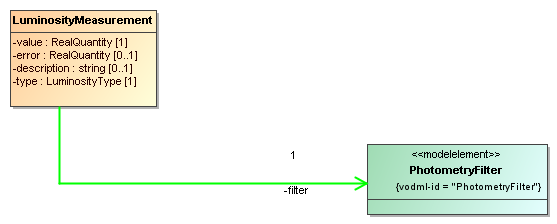
\includegraphics[width=4.64167in,height=1.86667in]{./media/image20.png}

Figure Reference (green arrow) from an ObjectTYpe to an ObjectType.

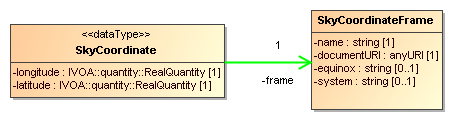
\includegraphics[width=3.76667in,height=0.99167in]{./media/image15.png}

Figure Reference from a DataType to an ObjectType

VO-DML/Schema

\textless xsd:complexType name=\emph{"Reference"}\textgreater{}

\textless xsd:complexContent\textgreater{}

\textless xsd:extension base=\emph{"Relation"/}\textgreater{}

\textless/xsd:extension\textgreater{}

\textless/xsd:complexContent\textgreater{}

\textless/xsd:complexType\textgreater{}

VO-DML/XML

\textless dataType\textgreater{}

\textless vodml-id\textgreater source.SkyCoordinate\textless/vodml-id\textgreater{}

\textless name\textgreater SkyCoordinate\textless/name\textgreater{}

...

\textless reference\textgreater{}

\textless vodml-id\textgreater source.SkyCoordinate.frame\textless/vodml-id\textgreater{}

\textless name\textgreater frame\textless/name\textgreater{}

\textless description\textgreater{}

...

\textless/description\textgreater{}

\textless datatype\textgreater{}

\textless vodml-ref\textgreater src:source.SkyCoordinateFrame\textless/vodml-ref\textgreater{}

\textless/datatype\textgreater{}

\textless multiplicity\textgreater1\textless/multiplicity\textgreater{}

\textless/reference\textgreater{}

...

\hypertarget{multiplicity}{%
\subsection{Multiplicity}\label{multiplicity}}

\textbf{Multiplicity} is used to indicate the cardinality of a
\textbf{Role} defined on an \textbf{ObjectType} or \textbf{DataType}. It
indicates how many values may be assigned to the role in an instance of
the type. VO-DML models this using the same terms as used in XML schema,
namely with a \textbf{minOccurs}/\textbf{maxOccurs} pair of values. The
former indicates the minimum number of instances or values that can be
assigned to a given role, the latter the maximum number. Also XMI
supports two values (named differently) and VO-DML follows its
specification in using -1 as a possible value for \textbf{maxOccurs}
that indicates that there is no limit on the possible number of
instances. In XML schema this is indicated using the string value
'unbounded', in UML diagrams generally with a '*'.

A special case is the assignment of a \textbf{Multiplicity} to an
\textbf{Attribute}. Users are strongly encouraged to only use the
following combinations of \textbf{minOccurs..maxOccurs}: 0..1,1..1 (or
simply 1), and 0..n, or n..n with n an explicit integer value
\textgreater1. For multiplicity greater than 1 the attribute must be
interpreted as an array of fixed size. To indicate that the value of
such an array attribute is optional, the multiplicity 0..n must be used
(i.e. minOccurs=0, maxOccurs=n). For maxOccurs n \textgreater{} 1,
minOccurs can only be 0 or n, other values are meaningless and illegal.

Modelers SHOULD NOT use open ended multiplicities, i.e. with
\textbf{maxOccurs}=-1, but it is not illegal in the current version of
this specification. \textbf{References} SHOULD NOT be given
multiplicities with \textbf{maxOccurs} \textgreater{} 1, but this is
allowed.\footnote{This is one way in which one might represent a UML
  \emph{aggregation} relationship, but preferably aggregation should be
  implemented using the pattern described in A.1 and illustrated in
  Figure 23.} This is one way in which one might represent a UML
\emph{aggregation} relationship, but preferably aggregation should be
implemented using the pattern described in A.1 and illustrated in Figure
23.

VO-UML

In VO-UML the multiplicity, when assigned to an attribute, shows up in
square brackets after the attribute's type. If minOccurs and maxOccurs
have the same value, that single value is shown. If they have different
values they show up separated by two dots, '..'. The value of -1 for
maxOccurs is represented by a '*':

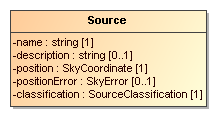
\includegraphics[width=1.8in,height=0.96667in]{./media/image16.png}

Figure Multiplicites assigned to attributes.

When the multiplicity is assigned to a relation, a similar pattern is
shown near the name of the relation, close to the target datatype of the
relation:

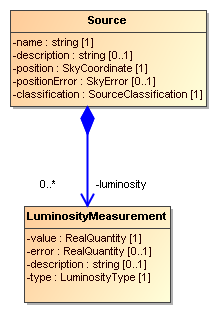
\includegraphics[width=1.8in,height=2.6in]{./media/image19.png}

Figure Multiplicity assigned to (composition) relation.

Note that the 0..* here indicates minOccurs = 0, maxOccurs = -1.

VO-DML/Schema

\textless xsd:complexType name=\emph{"Multiplicity"}\textgreater{}

\textless xsd:sequence\textgreater{}

\textless xsd:element name="minOccurs" type="xsd:nonNegativeInteger"

default=\emph{"1"/}\textgreater{}

\textless xsd:element name=\emph{"maxOccurs"} type=\emph{"xsd:int"}
default=\emph{"1"/}\textgreater{}

\textless/xsd:sequence\textgreater{}

\textless/xsd:complexType\textgreater{}

VO-DML/XML

\protect\hypertarget{_Type_extends_ReferencableElement}{}{}\textless objectType\textgreater{}

\textless vodml-id\textgreater source.Source\textless/vodml-id\textgreater{}

\textless name\textgreater Source\textless/name\textgreater{}

...

\textless attribute\textgreater{}

\textless vodml-id\textgreater source.Source.name\textless/vodml-id\textgreater{}

\textless name\textgreater name\textless/name\textgreater{}

...

\textless multiplicity\textgreater{}

\textless minOccurs\textgreater1\textless/minOccurs\textgreater{}

\textless maxOccurs\textgreater1\textless/maxOccurs\textgreater{}

\textless/multiplicity\textgreater{}

\textless/attribute\textgreater{}

...

\textless composition\textgreater{}

\textless vodml-id\textgreater source.Source.luminosity\textless/vodml-id\textgreater{}

\textless name\textgreater luminosity\textless/name\textgreater{}

...

\textless multiplicity\textgreater{}

\textless minOccurs\textgreater0\textless/minOccurs\textgreater{}

\textless maxOccurs\textgreater-1\textless/maxOccurs\textgreater{}

\textless/multiplicity\textgreater{}

\textless/composition\textgreater{}

\textless/objectType\textgreater{}

\hypertarget{minoccurs-nonnegativeinteger-0..1}{%
\subsubsection{minOccurs: nonnegativeInteger
{[}0..1{]}}\label{minoccurs-nonnegativeinteger-0..1}}

Indicates the minimum number of values that may be assigned to the
\textbf{Role} to which this \textbf{Multiplicity} is assigned. Must not
be larger than \textbf{maxOccurs} unless that has a negative value.
Default value 1.

\hypertarget{maxoccurs-integer-0..1}{%
\subsubsection{maxOccurs: integer
{[}0..1{]}}\label{maxoccurs-integer-0..1}}

Indicates the maximum number of values that may be assigned to the
\textbf{Role} to which this \textbf{Multiplicity} is assigned. Can only
take integer values \textgreater= -1. Must not be smaller than
\textbf{minOccurs} unless one assigns the value -1, which indicates that
there is no limit to the allowed number of values that may be assigned.
Default value 1.

\hypertarget{constraint}{%
\subsection{Constraint}\label{constraint}}

Apart from defining the basic structure in terms of types and their
interrelations, data models generally need to have explicit constraints
defined that restrict the possible objects and their interrelationships
or the values attributes may take in model instantiations. VO-DML has
some specialized support, particularly in multiplicity elements on roles
and the possibility of restricting attribute values through custom
enumerated types or the assignment of semantic concepts.

This first version of VO-DML provides support for constraints in a very
basic manner: a \textbf{Constraint} is only a named, referable element
whose \textbf{description} must be used to express the constraint in
natural language. It is anticipated that future versions of the language
will elaborate on this, adding for example an expression element in a
particular constraint specification language such as OCL {[}21{]},
possibly on specialized sub-types of Constraint. In VO-DML constraints
can only be added to a \textbf{Type}. If constraints are required for
\textbf{Roles} these must be defined on the containing type, or possibly
on a sub-type.

VO-UML

UML supports a
\href{http://www.uml-diagrams.org/constraint.html}{\emph{Constraint}}
element as a (possibly named) boolean expressions in some possibly
formal language, in particular OCL. In diagrams the constraint is
generally supposed to be placed close to the name of the element
containing it. In VO-UML this must always be the type.

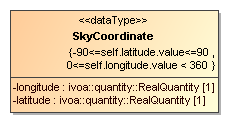
\includegraphics[width=2.375in,height=1.27083in]{./media/image21.png}

Figure Example of a constraint applied to a type. Here the language is
pseudo code, where \emph{self} follows the way OCL allows expressions to
refer to the instance of the type.

VO-DML/Schema

The XML schema only defines Constraint with a description element, which
MUST be used to define the constraint expression as a human readable
string, or possibly pseudo code if so desired.

\textless xsd:complexType name=\emph{"Constraint"}\textgreater{}

\textless xsd:sequence\textgreater{}

\textless xsd:element name="description" type="xsd:string

minOccurs="0"\emph{/}\textgreater{}

\textless/xsd:sequence\textgreater{}

\textless/xsd:complexType\textgreater{}

VO-DML/XML

\textless dataType\textgreater{}

\textless vodml-id\textgreater source.SkyCoordinate\textless/vodml-id\textgreater{}

\textless name\textgreater SkyCoordinate\textless/name\textgreater{}

...

\textless constraint\textgreater{}

\textless description\textgreater-90\&lt;=self.latitude.value\&lt;=90
\textless/description\textgreater{}

\textless/constraint\textgreater{}

\textless constraint\textgreater{}

\textless description\textgreater0\&lt;=self.longitude.value \&lt; 360
\textless/description\textgreater{}

\textless/constraint\textgreater{}

\textless attribute\textgreater{}

\textless vodml-id\textgreater source.SkyCoordinate.longitude\textless/vodml-id\textgreater{}

\textless name\textgreater longitude\textless/name\textgreater{}

...

\textless/attribute\textgreater{}

\textless attribute\textgreater{}

\textless vodml-id\textgreater source.SkyCoordinate.latitude\textless/vodml-id\textgreater{}

\textless name\textgreater latitude\textless/name\textgreater{}

...

\textless/attribute\textgreater{}

\hypertarget{subsettedrole-extends-constraint}{%
\subsection{SubsettedRole extends
Constraint}\label{subsettedrole-extends-constraint}}

A special class of constraints is defined for those restricting the
possible values of Roles defined on a type.

VO-UML

To define constraints on a \textbf{Role}, VO-UML uses UML's built-in
\textless\textless subsets\textgreater\textgreater{} concept. I.e. one
MUST redefine the \textbf{Role}, but declare it to be \emph{subsetting}
a role on the super-type. The \textbf{datatype} of the constrained Role
must be a subtype of its declared datatype. For clarity of
interpretation the redefined \textbf{Role} SHOULD use the same name, but
when deriving VO-DML/XML from the UML, the name is ignored (though it
may be used when generating the vodml-id for the role).

Other features of the constrained role may also be redefined as long as
the redefinition constrains the original set of values that is allowed
on the constrained Role.

The diagram shows subsetting of attributes. Here we make an extension to
the sample model where we pretend we have an AbstractSource that is
extended by 2 concrete sources, from the SDSS and 2MASS catalogues.
These subset the positionError attribute inherited from the super type.

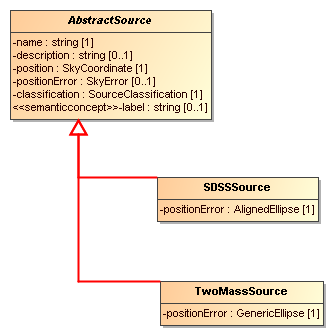
\includegraphics[width=3.46875in,height=3.48958in]{./media/image22.png}

Figure : Example of subsetting of a Role, here the Attribute
'positionError'. In the super type it is of type SkyError, in the
sub-types SDSSSource and TwoMassSource subsetted to AlignedEllipse and
GenericEllipse respectively, both of which extend SkyError.

VO-DML/Schema

\textless xsd:complexType name=\emph{"SubsettedRole"}\textgreater{}

\textless xsd:complexContent\textgreater{}

\textless xsd:extension base=\emph{"Constraint"}\textgreater{}

\textless xsd:sequence\textgreater{}

\textless xsd:element name=\emph{"role"}
type=\emph{"ElementRef"}/\textgreater{}

\textless xsd:element name=\emph{"datatype"} type=\emph{"ElementRef"}
minOccurs=\emph{"0"/}\textgreater{}

\textless xsd:element name=\emph{"semanticconcept"}
type=\emph{"SemanticConcept"}

minOccurs=\emph{"0"/}\textgreater{}

\textless/xsd:sequence\textgreater{}

\textless/xsd:extension\textgreater{}

\textless/xsd:complexContent\textgreater{}

\textless/xsd:complexType\textgreater{}

VO-DML/XML

\textless objectType\textgreater{}

\textless vodml-id\textgreater catalog.SDSSSource\textless/vodml-id\textgreater{}

\textless name\textgreater SDSSSource\textless/name\textgreater{}

\textless extends\textgreater{}

\textless vodml-ref\textgreater sample:catalog.AbstractSource\textless/vodml-ref\textgreater{}

\textless/extends\textgreater{}

\textbf{\textless constraint
xsi:type=\emph{"vo-dml:SubsettedRole"}\textgreater{}}

\textbf{\textless role\textgreater{}}

\textbf{\textless vodml-ref\textgreater{}}

\textbf{sample:catalog.AbstractSource.positionError}

\textbf{\textless/vodml-ref\textgreater{}}

\textbf{\textless/role\textgreater{}}

\textbf{\textless datatype\textgreater{}}

\textbf{\textless vodml-ref\textgreater sample:catalog.AlignedEllipse\textless/vodml-ref\textgreater{}}

\textbf{\textless/datatype\textgreater{}}

\textbf{\textless/constraint\textgreater{}}

\textless/objectType\textgreater{}

Since \textbf{Type} only has a \textbf{constraint} collection of type
Constraint, in the XML one must use the xsi:type mechanism to indicate
that a particular sub-type is used, here \textbf{vo-dml:SubsettedRole}.

\hypertarget{role-elementref}{%
\subsubsection{role: ElementRef}\label{role-elementref}}

Identifies the role that is subsetted. This Role MUST be available on
the type owning the constraint, i.e. it MUST be defined on the type
itself or on one of its super-types.

\hypertarget{datatype-elementref-1}{%
\subsubsection{\texorpdfstring{datatype:
\protect\hyperlink{elementref}{ElementRef}}{datatype: ElementRef}}\label{datatype-elementref-1}}

The \textbf{datatype} element can be used to indicate that the datatype
of the subsetted \textbf{Role} MUST be a sub-type of the datatype
declared for the Role itself. In the interpretation of Type-s as sets of
instances, subtypes define subsets, which explains the name of this
element. This is a common design pattern and directly borrowed from UML,
where it is used as stereotype on a redefinition of the role. We use a
special \textbf{Constraint} to support the same concept. Redefining the
\textbf{Role} would require defining a new vodml-id. This would
complicate the implementation of simple clients that look for instances
of the \textbf{Role}, but are agnostic about the precise type of the
owning \textbf{Type}.

\hypertarget{semanticconcept-semanticconcept}{%
\subsubsection{semanticconcept:
SemanticConcept}\label{semanticconcept-semanticconcept}}

The super type may have defined a semantic concept for the Role or not.
This attribute allows either to define the assignement of semantic
concept to the subtype in the latter case or to restrict the values to a
narrower concept than that assigned to it on the super-type when the
role on the supertype already has a semantic concept with a topConcept
defined on it. But also, when the \textbf{Role} on the super-type
already has a \textbf{semanticconcept} with a \textbf{topConcept}
defined on it, the subtype may restrict the values to a narrower concept
than that assigned to it on the super-type.

\hypertarget{the-ivoa-base-model-normative}{%
\section{\texorpdfstring{The \emph{ivoa} base model
{[}Normative{]}}{The ivoa base model {[}Normative{]}}}\label{the-ivoa-base-model-normative}}

Ultimately all types in a VO-DML model are defined as hierarchies of
primitive types. This spec defines a special, predefined model (with
name='ivoa') that contains a set of the most common of such types:
integer, real, string etc. This model SHOULD be imported by all other
models and its types SHOULD be used for the leaf attributes of object
types and data types, or as ultimate super-types of custom primitive
types. The use of such a standardized \emph{model} and its types
provides interoperability between models and allows the definition of
standard serialization strategies. By defining these as types in a
model, rather than predefined enumeration for example, modelers can
create their own extensions and specializations through inheritance.
These can then in principle still be recognized by interpreters that
understand the common base model.

Apart from the primitive types, the \emph{ivoa} model also defines some
structured data types for representing \emph{quantities}, values with
units. Making these part of the standard allows one to make some special
arrangements for mapping quantity-like attributes to FIELD-s and PARAM-s
in VOTable and is used in the Mapping specification {[}3{]}.

The diagram in Figure 21 shows the types defined in this model. Its
formal VO-DML/XML representation can be found in

\url{http://www.ivoa.net/xml/VODML/IVOA-v1.vo-dml.xml}.

Note, the vodml-id of all types exactly follow the generation rules in
Appendix C. E.g. to refer to the 'string' type one should always use the
vodml-ref 'ivoa:string'

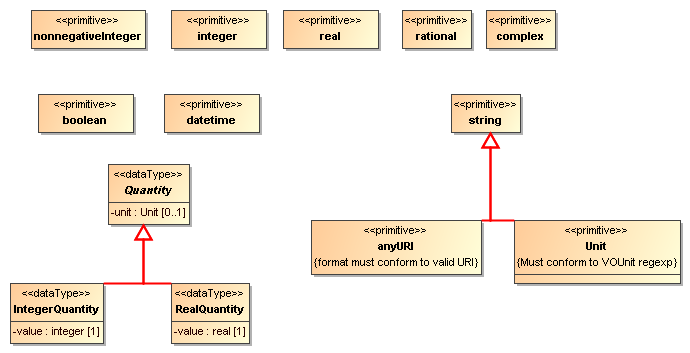
\includegraphics[width=6in,height=3.06956in]{./media/image23.png}

Figure VO-UML diagram with the types from the basic 'ivoa' data model.

Note that the numeric types in this model are defined to correspond to
the mathematical number types\(\mathbb{N}\), \(\mathbb{Z}\),
\(\mathbb{Q}\), \(\mathbb{R}\) and \(\mathbb{C}\), rather than to a
serialization format understandable to standard programming languages or
database systems. Hence it contains only 'integer' rather than (4 byte)
'int', (2 byte) 'short', and/or (8 byte)'long'. Similarly it contains
'real' rather than 'float' or 'double( precision)'. This allows one to
assign types to an attribute based on its semantics, rather than on
application specific considerations. When using the model to annotate
instances in a serialization, or representing its types in software,
concrete types will have to be used. One may expect that these should be
compatible with the datatype of the attribute, but any possible formal
restrictions on the serializations of these types are beyond the scope
of this specification and are deferred to a possible mapping
specification.

Here we list the types and describe them.

\hypertarget{nonnegativeinteger}{%
\subsection{nonnegativeInteger}\label{nonnegativeinteger}}

Represents integers\textgreater=0, elements of \(\mathbb{N}\).

\hypertarget{integer}{%
\subsection{integer}\label{integer}}

Represents all integers, elements of \(\mathbb{Z}\).

\hypertarget{rational}{%
\subsection{rational}\label{rational}}

Represents all rational numbers, elements of \(\mathbb{Q.}\) A
serialization format is not specified for this datatype that is not
commonly encountered in computer languages.

\hypertarget{real}{%
\subsection{real}\label{real}}

Represents all real numbers, elements of \(\mathbb{R}\).

\hypertarget{complex}{%
\subsection{complex}\label{complex}}

Represents all complex numbers, elements of \(\mathbb{C.}\) A
serialization format is not specified.

\hypertarget{boolean}{%
\subsection{boolean}\label{boolean}}

The standard datatype representing the logical values \textbf{true} and
\textbf{false}. In serializations these may be represented in different
ways such as 0 and 1 or T and F for example.

\hypertarget{datetime}{%
\subsection{datetime}\label{datetime}}

Represents a point in time. Will generally need time frame and units in
the serialization. Can also be used for \textbf{Attributes} just needing
a time without a date part and vice versa.

\hypertarget{string}{%
\subsection{string}\label{string}}

A standard string type, consisting of zero or more characters. We define
string as a primitive type (such as in Java), rather than as an array of
characters (as in VOTable for example).

\hypertarget{anyuri-extends-string}{%
\subsection{anyURI extends string}\label{anyuri-extends-string}}

A special subtype of string representing uniform resource
identifiers\footnote{https://tools.ietf.org/html/rfc3986}. Inspired by
XML-Schema's anyURI\footnote{http://www.w3.org/TR/xmlschema-2/\#anyURI}
type.

\hypertarget{unit-extends-string}{%
\subsection{Unit extends string}\label{unit-extends-string}}

A string representing a unit following the IVOA specification in
{[}27{]} for representing units as strings.

\hypertarget{quantity}{%
\subsection{\texorpdfstring{\emph{Quantity}}{Quantity}}\label{quantity}}

A number with a unit. We predefine this type and its two sub-types to
represent the pattern that in scientific data models numerical values
very often will have to be represented by a literal number and a unit. A
particular motivation for defining this concept in the base model is its
use in the mapping specification, which allows mapping of these
structured DataType-s directly to single FIELDs or PARAMs. Here the unit
specified on those VOTable elements is assumed to be mapped to the unit
on the Quantity \textbf{Attribute}.

\hypertarget{unit-unit}{%
\subsubsection{unit : Unit}\label{unit-unit}}

This attribute represents the unit that is to be assigned to the
numerical value. The unit must be a string conforming to the unit
specification represented by the
\protect\hyperlink{unit-extends-string}{ivoa:Unit} type.

\hypertarget{integerquantity-extends-quantity}{%
\subsection{IntegerQuantity extends
Quantity}\label{integerquantity-extends-quantity}}

A quantity representing an integer value with a unit.

\hypertarget{value-integer}{%
\subsubsection{\texorpdfstring{ value:
integer}{ value: integer}}\label{value-integer}}

The attribute holding on to the numerical value for this Quantity. This
value must be an \protect\hyperlink{integer}{ivoa:integer}.

\hypertarget{realquantity-extends-quantity}{%
\subsection{RealQuantity extends
Quantity}\label{realquantity-extends-quantity}}

A quantity where the value is a real number.

\hypertarget{value-real}{%
\subsubsection{value: real}\label{value-real}}

The attribute holding on to the numerical value for this Quantity. This
value must be an \protect\hyperlink{real}{ivoa:real.}

\hypertarget{procedure-for-defining-data-models-in-the-ivoa}{%
\section{Procedure for defining data models in the
IVOA}\label{procedure-for-defining-data-models-in-the-ivoa}}

\hypertarget{ivoa-standardized-data-models}{%
\subsection{IVOA-standardized data
models}\label{ivoa-standardized-data-models}}

A data model specified in VO-DML can be endorsed by the IVOA to become a
standard data model. A standard data model consists of at least three
artifacts:

\begin{itemize}
\item
  A standard text adopted by the IVOA according to the rules laid down
  in the IVOA document standard {[}30{]}. This must at least discuss use
  cases and the general design of the model. The level of detail to
  which individual data model items are discussed in the standard text
  is up to the authors. The authoritative source on these details always
  is the VO-DML/XML source. When adding UML-like diagrams or diagram
  snippets in this text, it strongly suggested that modelers use the
  VO-UML examples as described in Appendix A and used in examples
  throughout the current document.
\item
  The data model itself, written in VO-DML/XML, which MUST conform to
  the VO-DML schema\footnote{http://www.ivoa.net/xml/VODML/vo-dml-v1.xsd}
  and the rules in the VO-DML Schematron file\footnote{\url{http://www.ivoa.net/xml/VODML/vo-dml-v1.sch.xml}}.
\item
  A detailed documentation in HTML format containing human-readable
  definitions for all elements of the data model, formatted in HTML and
  furnished with HTML-accessible anchors (a/@name or @id attributes) for
  the vodml-refs contained in the data model. The intent is that the
  data model URL with an element's vodml-id as a fragment identifier
  will lead to element-specific documentation.
\end{itemize}

When a standard data model reaches the status of Proposed
Recommendation, the VO-DML document and the HTML are made available in
the IVOA document repository at their final URLs. They may, however, be
modified there without further notice until the document reaches REC
status.

At the same time, a StandardsRegExt {[}31{]} document for the standard
is uploaded to (or, for updated models, updated in) in the Registry.
Additionally, registry records for the data model(s) contained in a
standard must be uploaded to (or updated in) the registry. This record
must be of the type vodm:DataModel, where vodm is the canonical prefix
assigned to the namespace

http://www.ivoa.net/xml/DataModel/v1;

As usual for VO schema files produced by the IVOA, retrieving the
namespace URL yields the current schema file.

The identifiers for IVOA data model records should be of the form

ivo://ivoa.net/std/\textless dmname\textgreater dm.

In addition to basic VOResource metadata, DataModels define the
following extra metadata in direct children of the resource element:

\begin{itemize}
\item
  dm-prefix - The prefix claimed by the model.
\item
  dm-uri - The URI at which to retrieve the VO-DML definition of the
  model.
\end{itemize}

In RegTAP, these pieces of data are kept in the rr.res\_details table
with keys formed in parallel to those defined in RegTAP; hence, prefixes
are found under /dm-prefix, URI is under /dm-uri. For instance, to
retrieve a data model URI for a given prefix, the corresponding RegTAP
query would be:

SELECT b.detail\_value

FROM rr.res\_detail AS a

JOIN rr.res\_detail AS b USING (ivoid)

WHERE a.detail\_xpath='/dm-prefix'

AND a.detail\_value='ivoa'

AND b.detail\_xpath='/dm-uri'

The standard(s) that define the data model SHOULD be given in an
IsSupplementTo relationship.

Note that this allows Registry clients to support use cases like:

\begin{itemize}
\item
  Locate the specification for a data model based on either prefix or
  URI
\item
  Ascertain that a chosen prefix is not being used by another data model
\item
  Find the URI for a DM prefix.
\end{itemize}

\hypertarget{other-registered-data-models}{%
\subsection{Other registered data
models}\label{other-registered-data-models}}

Data providers can register their application-specific data models
without going through an IVOA review process. In that case, only two
artifacts have to be publicly available, preferably on a web server
under the provider's control:

\begin{itemize}
\item
  The data model itself, written in VO-DML.
\item
  A detailed documentation in HTML format containing human-readable
  definitions for all elements of the data model, formatted in HTML and
  furnished with HTML-accessible anchors (a/@name or @id attributes) for
  the vodml-refs contained in the data model. The intent is that the
  data model URL with an element's vodml-id as a fragment identifier
  will lead to element-specific documentation. It is recommended to
  generate this HTML document from the VO-DML using the vo-dml2html.xsl
  script documented on the IVOA wiki:
\end{itemize}

\url{http://wiki.ivoa.net/twiki/bin/view/IVOA/VodmlResources}.

As in 6.1 , the party defining the data model constructs a
DataModel-typed registry record defining dm-prefix and dm-uri. Again, a
document giving motivation, use cases, and the like SHOULD be given in
an \textbf{isSupplementTo} relationship. The registry record can be
uploaded through any publishing registry.

\hypertarget{suggestions}{%
\subsection{Suggestions}\label{suggestions}}

Non-normative guidelines how to build a model, and criteria on what
makes a "good" model.

\begin{itemize}
\item
  Decide \emph{why} one wants to create a data model, what is its goal.
  This includes defining what \emph{kind} of data model should be
  created. Default goal for any IVOA data model should be that it allows
  existing and future databases to describe their contents (at least
  partially) in terms of the model, which should serve as what is often
  called a \emph{global schema}. In certain cases a model may be
  developed to provide support for a particular application area, for
  example when defining a data access protocol. Here one can decide to
  support faithful serialization of data models in targeted XML
  documents as well as annotated serialization in VOTable. Such models
  may not necessarily be reusable, but often they can be seen as
  derivations of, \emph{views of}, one or more fundamental data models
  that \emph{were} defined for reusability purposes.
\item
  Decide on universe of discourse: what concepts must be described? How
  rich should the model be?
\item
  Create a conceptual/logical model. In drawings on whiteboard
  ("VO-UML"), then transcribe to VO-DML/XML. Define concepts completely,
  realizing that applications may pick and choose and transform.
\end{itemize}

Sometimes, in application contexts: derive one or more physical
representations. Use as much as possible standard, if possible automated
derivation methods of VO-DML to target representation.

\hypertarget{references}{%
\section{References}\label{references}}

\begin{enumerate}
\def\labelenumi{\arabic{enumi}.}
\item
  Abiteboul etal 2011 \emph{Web Data Management}\\
  Online version at \url{http://webdam.inria.fr/Jorge/files/wdm.pdf} )
\item
  Ullman, \emph{Information Integration Using Logical Views\\
  }ICDT '97 Proceedings of the 6\textsuperscript{th} International
  Conference on Database Theory p19-40. Springel-Verlag London, UK
  ©1997. \url{http://ilpubs.stanford.edu:8090/154/1/1996-28.pdf}
\item
  \emph{Standard serialization of Data Models in VOTable}, in
  preparation. Follow progress on DM working group page
  \url{http://wiki.ivoa.net/twiki/bin/view/IVOA/IvoaDataModel}
\item
  \emph{VOTable Format Definition Version 1.3}\\
  \url{http://www.ivoa.net/documents/VOTable/20130920/}
\item
  \emph{Table Access Protocol Version 1.0}\\
  \url{http://www.ivoa.net/documents/TAP/20100327/}
\item
  \emph{An IVOA Standard for Unified Content Descriptors Version 1.10\\
  }\url{http://www.ivoa.net/documents/latest/UCD.html}
\item
  \emph{The UCD1+ Controlled Vocabulary Version 1.23\\
  }\url{http://www.ivoa.net/documents/cover/UCDlist-20070402.html}
\item
  \emph{Simulation Data Model Version 1.0}\\
  \url{http://www.ivoa.net/documents/SimDM/20120503/index.html}
\item
  \emph{Referencing STC in VOTable\\
  }http://www.ivoa.net/documents/Notes/VOTableSTC/
\item
  \url{http://www.schematron.com/}
\item
  \url{http://www.ivoa.net/documents/SimDM/index.html}
\item
  \url{http://www.omg.org/spec/UML}
\item
  http://www.omg.org/spec/UML/2.4.1/Superstructure/PDF/
\item
  \url{http://vo-urp.googlecode.com/}
\item
  \url{http://www.omg.org/spec/XMI/2.1/}
\item
  \url{http://www.uml-diagrams.org/}
\item
  Gray \emph{etal} 2009 \emph{Vocabularies in the Virtual Observatory}\\
  IVOA recommendation 07 October 2009,
  \url{http://www.ivoa.net/documents/latest/Vocabularies.html}
\item
  Ecore:
  \href{http://download.eclipse.org/modeling/emf/emf/javadoc/2.9.0/org/eclipse/emf/ecore/package-summary.html\#details}{http://download.eclipse.org/modeling/emf/emf/javadoc/2.9.0/org/eclipse/emf/ecore/package-summary.html}
\item
  OWL2: \url{http://www.w3.org/TR/owl2-overview/}
\item
  RDF-Schema: \url{http://www.w3.org/TR/rdf-schema/}
\item
  Object Constraint Language
  \url{http://www.omg.org/spec/OCL/2.4/PDF}2.4/PDF
\item
  \emph{Utypes: current usages and practices in the IVOA}
  \url{http://www.ivoa.net/documents/Notes/UTypesUsage/index.html}
\item
  \emph{Simple Spectral Access Protocol Version 1.1}
  \url{http://www.ivoa.net/documents/SSA/}
\item
  XML Schema Part 2: Datatypes Second Edition
  \url{http://www.w3.org/TR/xmlschema-2/}
\item
  \emph{Observation Data Model Core Components and its Implementation in
  the Table Access Protocol Version 1.0
  \url{http://www.ivoa.net/documents/ObsCore/20111028/index.html}}
\item
  Meilir Page-Jones \emph{Fundamentals of Object-Oriented Design in UML}
  Addison-Wesley 2000.
\item
  \emph{Units in the VO Version 1.0}
  \href{http://www.ivoa.net/documents/VOUnits/index.html}{\emph{http://www.ivoa.net/documents/VOUnits/index.html}}
\item
  \emph{IVOA Identifiers, version 2.0\\
  }\url{http://www.ivoa.net/documents/IVOAIdentifiers/}
\item
  \emph{XML Schema Versioning Policies Version 1.0\\
  }\url{http://www.ivoa.net/documents/Notes/XMLVers/20160906/PEN-schemaVersioning-1.0-20160906.pdf}
\item
  \emph{IVOA Document Standards Version 1.2}
  \url{http://www.ivoa.net/documents/DocStd/20100413/}
\item
  \emph{Standards RegExt: a VOResource Schema Extension for Describing
  IVOA Standards Version 1.0\\
  }\url{http://www.ivoa.net/documents/StandardsRegExt/}
\end{enumerate}

\hypertarget{relation-to-uml}{%
\section{Relation to UML}\label{relation-to-uml}}

The following table summarizes the relation between VO-DML and UML. It
lists for each major VO-DML concept the corresponding UML concept or
concepts and, where appropriate, gives the graphical symbol that SHOULD
be used in VO-UML. The UML concepts, generally referred to as
MetaClasses, have a reference to a paragraph in the UML specification
version 2.4.1 {[}13{]} and are also hyperlinked to a more readable
definition in \href{http://www.uml-diagrams.org}{www.uml-diagrams.org}.
Below the table we discuss some UML meta-types that we have \emph{not}
included in VO-DML and motivate our decision.

\begin{longtable}[]{@{}
  >{\raggedright\arraybackslash}p{(\columnwidth - 4\tabcolsep) * \real{0.2198}}
  >{\raggedright\arraybackslash}p{(\columnwidth - 4\tabcolsep) * \real{0.3609}}
  >{\raggedright\arraybackslash}p{(\columnwidth - 4\tabcolsep) * \real{0.4193}}@{}}
\toprule
\begin{minipage}[b]{\linewidth}\raggedright
\textbf{VO-DML concept}
\end{minipage} & \begin{minipage}[b]{\linewidth}\raggedright
\textbf{Relevant UML MetaClass(es)}
\end{minipage} & \begin{minipage}[b]{\linewidth}\raggedright
\textbf{VO-UML graphical notation}
\end{minipage} \\
\midrule
\endhead
\protect\hyperlink{model}{\textbf{Model}} &
\href{http://www.uml-diagrams.org/package-diagrams/model.html}{Model}
§17.3.1 &
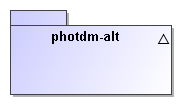
\includegraphics[width=1.53333in,height=0.86667in]{./media/image9.png} \\
\protect\hyperlink{modelimport}{\textbf{ModelImport}} &
\href{http://www.uml-diagrams.org/package-diagrams/model.html}{Model}
§17.3.1

\href{http://www.uml-diagrams.org/package-diagrams.html\#package-import}{PackageImport}
§7.3.40

\href{http://www.uml-diagrams.org/package-diagrams.html\#element-import}{ElementImport}
§7.3.15 & \\
\protect\hyperlink{referableelement}{\emph{\textbf{ReferableElement}}} &
\href{http://www.uml-diagrams.org/uml-core.html\#named-element}{NamedElement}
§7.3.34 & \\
\protect\hyperlink{package-extends-referableelement}{\textbf{Package}} &
\href{http://www.uml-diagrams.org/package-diagrams.html\#package}{Package}
§7.3.38 &
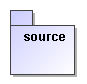
\includegraphics[width=0.725in,height=0.7in]{./media/image24.png} \\
\protect\hyperlink{type-extends-referableelement}{\emph{\textbf{Type}}}
& \href{http://www.uml-diagrams.org/uml-core.html\#type}{Type} §7.3.52

\href{http://www.uml-diagrams.org/classifier.html}{Classifier} §7.3.8
& \\
\protect\hyperlink{_extends:_ElementRef}{\textbf{\emph{Type}.extends}} &
\href{http://www.uml-diagrams.org/generalization.html}{Generalization}
§7.3.20 &
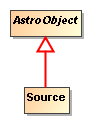
\includegraphics[width=0.75833in,height=1.025in]{./media/image25.png} \\
\protect\hyperlink{objecttype-extends-type}{\textbf{ObjectType}} &
\href{http://www.uml-diagrams.org/class-diagrams.html\#class}{Class}
§7.3.7 &
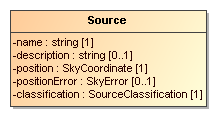
\includegraphics[width=1.8in,height=0.96667in]{./media/image16.png} \\
\protect\hyperlink{valuetype-extends-type}{\emph{\textbf{ValueType}}} &
\href{http://www.uml-diagrams.org/class-diagrams.html\#data-type}{DataType}
§7.3.11 & \\
\protect\hyperlink{datatype-extends-valuetype}{\textbf{DataType}} &
\href{http://www.uml-diagrams.org/class-diagrams.html\#data-type}{DataType}
§7.3.11 &
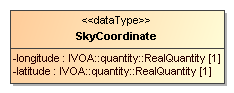
\includegraphics[width=1.95in,height=0.775in]{./media/image26.png} \\
\protect\hyperlink{primitivetype-extends-valuetype}{\textbf{PrimitiveType}}
&
\href{http://www.uml-diagrams.org/class-diagrams.html\#primitive-type}{PrimitiveType}
§7.3.44 &
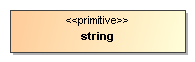
\includegraphics[width=1.625in,height=0.51667in]{./media/image27.png} \\
\protect\hyperlink{enumeration-extends-valuetype}{\textbf{Enumeration}}
&
\href{http://www.uml-diagrams.org/class-diagrams.html\#enumeration}{Enumeration}
§7.3.16 &
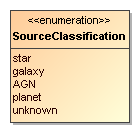
\includegraphics[width=1.15833in,height=1.1in]{./media/image14.png} \\
\protect\hyperlink{_Literal}{\textbf{EnumLiteral}} & EnumerationLiteral
§7.3.17 & See Enumeration above \\
\protect\hyperlink{role-extends-referableelement}{\emph{\textbf{Role}}}
& \href{http://www.uml-diagrams.org/uml-core.html\#feature}{Feature}
§7.3.19

\href{http://www.uml-diagrams.org/uml-core.html\#structural-feature}{StructuralFeature}
§7.3.50

\href{http://www.uml-diagrams.org/uml-core.html\#type}{TypedElement}
§7.3.53

\href{http://www.uml-diagrams.org/property.html}{Property} §7.3.45 & \\
\protect\hyperlink{attribute-extends-role}{\textbf{Attribute}} &
\href{http://www.uml-diagrams.org/property.html}{Property} §7.3.45 & See
ObjectType and DataType above. \\
\protect\hyperlink{relation-extends-role}{\emph{\textbf{Relation}}} &
\href{http://www.uml-diagrams.org/association.html}{Association} §7.3.3

\href{http://www.uml-diagrams.org/association.html\#association-end}{AssociationEnd}

\href{http://www.uml-diagrams.org/property.html}{Property} §7.3.45 & \\
\protect\hyperlink{reference-extends-relation}{\textbf{Reference}} &
\href{http://www.uml-diagrams.org/association.html}{Association} §7.3.3

\href{http://www.uml-diagrams.org/association.html\#association-end}{AssociationEnd}

\href{http://www.uml-diagrams.org/property.html}{Property} §7.3.45 &
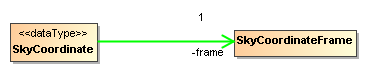
\includegraphics[width=3.05in,height=0.59167in]{./media/image28.png} \\
\protect\hyperlink{composition-extends-relation}{\textbf{Composition}} &
\href{http://www.uml-diagrams.org/association.html}{Association} §7.3.3

\href{http://www.uml-diagrams.org/association.html\#association-end}{AssociationEnd}

\href{http://www.uml-diagrams.org/property.html}{Property} §7.3.45

AggregationKind §7.3.2 &
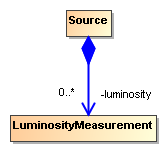
\includegraphics[width=1.38333in,height=1.25833in]{./media/image29.png} \\
\protect\hyperlink{multiplicity}{\textbf{Multiplicity}} &
\href{http://www.uml-diagrams.org/multiplicity.html}{Multiplicity} § &
See annotation in diagram for attributes, reference, composition \\
\protect\hyperlink{constraint}{\textbf{Constraint}} &
\href{http://www.uml-diagrams.org/constraint.html}{Constraint} §7.3.10
& \\
\protect\hyperlink{subsettedrole-extends-constraint}{\textbf{SubsettedRole}}
& Property.subsettedProperty, Propery.redefinedProperty §7.3.45 & \\
\protect\hyperlink{semanticconcept}{\textbf{SemanticConcept}} & &
\begin{minipage}[t]{\linewidth}\raggedright
\textless\textless semanticconcept\textgreater\textgreater{} with tags:

topConcept\\
vocabularyURI\strut
\end{minipage} \\
\bottomrule
\end{longtable}

UML meta-classes not included in VO-DML

Aggregation

A common question is why UML's
\href{http://www.uml-diagrams.org/association.html\#shared-aggregation}{\emph{Aggregation}}
meta-class (see §7.3.2 and §7.3.3) has not been included in VO-DML.
Aggregation is a kind of shared relationship between a whole and a part.
It is "shared" in that the part can be a part in multiple "wholes" at
the same time, in contrast to a composition relationship. Consequently
the part's life cycle is not tied to that of any "whole".

In UML this relation is represented graphically by a line with an open
diamond as in Figure 22.

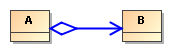
\includegraphics[width=2.40625in,height=0.71765in]{./media/image30.png}

Figure UML Aggregation relationship.

We have excluded \emph{Aggregation} for the following reasons

\begin{enumerate}
\def\labelenumi{\arabic{enumi}.}
\item
  In virtually all situations an aggregation can be represented by the
  pattern illustrated in Figure 23. In fact, in almost all cases we have
  encountered where an aggregation \emph{was} used, the relation between
  the types A and B was actually better modelled by that pattern as more
  attributes were desirable to describe the relation in more detail;
  i.e. it needed a separate type to represent the relation fully.
\item
  The representation of the shared aggregation pattern in a relational
  database, arguably an important use case, requires a separate table
  playing basically the role of the type AB in Figure 23. This is in
  contrast to the case of the composition relationship, where a foreign
  key from part-to-whole is the natural representation. To make the
  mapping explicit, it is useful to enforce that types exist also in
  VO-DML. This is especially important if we wish to be able to annotate
  such a database pattern with data model information. There it is
  useful if each element in the physical representation has a 1-1
  relation to an element in the model.
\item
  The wish to keep the language as simple and non-redundant as possible.
  This is obviously convenient for clients of the model, which require
  less code to take care of all cases. When different methods exist to
  implement the same pattern, different choices will be made, with the
  possibility of confusion and the need for clients that are more
  sophisticated. In the case of Aggregation moreover it has been noticed
  that it is prone to errors in the model, inducing inexperienced
  modelers to ignore important model components.
\end{enumerate}

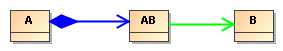
\includegraphics[width=3.0478in,height=0.54925in]{./media/image31.png}

Figure VO-DML aggregation pattern.

Summarizing, there is only a very small percentage of cases where
aggregation would really be sufficient. It seems never necessary. In
those cases where it would be used it would obfuscate the relationship
between the model and arguably its most important physical
representation, namely relational databases. It adds redundancy to a
language that for many first-time users is hard enough to use as it is,
and would complicate the work of coders of client software. That in some
cases an extra type must be added to a model was considered a small
price to pay for these advantages.

Double inheritance

VO-DML does not support multiple inheritance. In this it follows
computer languages such as Java and C\# (though not C++ or Python) and
XML schema. The main aim of our restriction is to promote simplicity of
mapping models to important serializations and trying to limit the abuse
of inheritance that even with single inheritance is very common (see
e.g. Chapter 12 in {[}26{]}).

\hypertarget{mapping-to-serialization-meta-models}{%
\section{\texorpdfstring{Mapping to serialization meta-models
}{Mapping to serialization meta-models }}\label{mapping-to-serialization-meta-models}}

This appendix contains examples how one might map a VO-DML data model to
a physical representation format described by its own meta-model. These
mappings aim to be as close to 1-1 as possible, providing so called
\emph{faithful} representations of the model. Developing standards for
mappings to languages like these could greatly simplify a modeling
process, as one need only define the conceptual model itself and use
automated procedures to derive the serialization formats.

XSD

\begin{longtable}[]{@{}
  >{\raggedright\arraybackslash}p{(\columnwidth - 2\tabcolsep) * \real{0.5000}}
  >{\raggedright\arraybackslash}p{(\columnwidth - 2\tabcolsep) * \real{0.5000}}@{}}
\toprule
\begin{minipage}[b]{\linewidth}\raggedright
\textbf{VO-DML concept}
\end{minipage} & \begin{minipage}[b]{\linewidth}\raggedright
\textbf{XSD concept}
\end{minipage} \\
\midrule
\endhead
ObjectType & complexType \\
DataType & complexType \\
Enumeration & simpleType with restriction list elements for the
EnumLiterals \\
PrimitiveType & simpleType, possibly with restriction \\
Attribute & element on complexType, type corresponding to mapping of
datatype \\
Composition & element on complexType, type corresponding to mapping of
datatype \\
Reference & element on complexType, type must be able to perform remote
referencing, possibly an xlink, or an element of a special purpose type
designed for referencing. \\
Type.extends & xsd:extension for ObjectType and DataType,
xsd:restriction for PrimitiveType and Enumeration. \\
Package & targetNamespace if each package is defined in its own
document. \\
\bottomrule
\end{longtable}

Relational databases

Follow typical Object-Relational mapping rules.

\begin{longtable}[]{@{}
  >{\raggedright\arraybackslash}p{(\columnwidth - 2\tabcolsep) * \real{0.3323}}
  >{\raggedright\arraybackslash}p{(\columnwidth - 2\tabcolsep) * \real{0.6677}}@{}}
\toprule
\begin{minipage}[b]{\linewidth}\raggedright
\textbf{VO-DML concept}
\end{minipage} & \begin{minipage}[b]{\linewidth}\raggedright
\textbf{RDB concept}
\end{minipage} \\
\midrule
\endhead
ObjectType & Table \\
DataType & Used as data type of Attributes, mapped to one or more
Columns in a Table. \\
Enumeration & Used as data type of Attributes, mapped to one Column in a
Table \\
PrimitiveType & Used as data type of Attributes, mapped to one Column in
a Table \\
Attribute & One or more Columns in a Table depending on datatype \\
Composition & Foreign key from child to parent Table \\
Reference & Foreign key from referrer to referent. \\
Type.extends & Depending on inheritance mapping strategy\footnote{E.g.
  see \url{http://en.wikibooks.org/wiki/Java_Persistence/Inheritance}}
this can be a foreign key from a Table representing the sub-type to the
one representing the base type. Or may lead to sub-type Columns being
added to table for super-type. \\
Package & Could be mapped to a Schema, but should have no nested
packages as nesting of schemas is not supported in RDBs. \\
\bottomrule
\end{longtable}

Java

VO-DML maps pretty much 1-1 to an OO language like Java. An automated
generation of Java classes is very well possible as show by the VO-URP
proto-type used in the Simulation Data Model {[}8{]} effort.

\begin{longtable}[]{@{}
  >{\raggedright\arraybackslash}p{(\columnwidth - 2\tabcolsep) * \real{0.3323}}
  >{\raggedright\arraybackslash}p{(\columnwidth - 2\tabcolsep) * \real{0.6677}}@{}}
\toprule
\begin{minipage}[b]{\linewidth}\raggedright
\textbf{VO-DML concept}
\end{minipage} & \begin{minipage}[b]{\linewidth}\raggedright
\textbf{Java concept}
\end{minipage} \\
\midrule
\endhead
ObjectType & class \\
DataType & class \\
Enumeration & enum \\
PrimitiveType & Appropriate built in primitive type (int, boolean,
float, etc) or corresponding class, otherwise a custom class. \\
Attribute & Attribute in class of appropriate type. \\
Composition & Collection\textless T\textgreater{} attribute on parent
class, with T the type corresponding to the child type. \\
Reference & Attribute in class of Java type corresponding to the data
type of the reference. \\
Type.extends & class \textless sub-type\textgreater{} extends
\textless super-type\textgreater{} \\
Package & Java package, hierarchical with maybe some root package
representing the model. \\
\bottomrule
\end{longtable}

\hypertarget{vodml-id-generation-rules}{%
\section{\texorpdfstring{vodml-id generation rules
}{vodml-id generation rules }}\label{vodml-id-generation-rules}}

The only requirement on the
\textless{}\protect\hyperlink{vodml-id-vodmlid-1}{vodml-id}\textgreater{}
identifying model elements is that it is unique within the context of
the model. However, it may be useful for such IDs to be human-readable,
so to intuitively provide information about the elements they identify.
This specification states that vodml-id SHOULD be made human-readable
according to specific rules that represent the location of the
identified element in the model, encoded in the grammar presented below.

In the past\footnote{The Simulation Data Model
  {[}http://ivoa.net/documents/SimDM/20120503{]} provided such a grammar
  for the first time for the list of utypes accompanying that model.}
rules have been defined for generating such unique identifiers for
elements in a data model, and the following grammar is built starting
from that previous attempt. Note that uniqueness depends on rules on the
uniqueness of names in a particular context, here represented by a
location in a hierarchy:

vodml-id := package-vodml-id \textbar{} type-vodml-id \textbar{}

attribute-vodml-id \textbar{} composition-vodml-id \textbar{}

reference-vodml-id \textbar{} container-vodml-id

package-vodml-id := \textless package-name\textgreater{} {[}``.''
\textless package-name\textgreater{]}*

type-vodml-id := {[}package-vodml-id ``.''{]}
\textless type-name\textgreater{}

attribute-vodml-id := type-vodml-id ``.''
\textless attribute-name\textgreater{}

composition-vodml-id :=

type-vodml-id ``.'' \textless composition-name\textgreater{}

reference-vodml-id := type-vodml-id ``.''
\textless reference-name\textgreater{}

container-vodml-id := ``vo-dml:Object.CONTAINER''

vodml-ref := \textless model-name\textgreater{} ``:'' vodml-id

The grammar for the vodml-ref reference to an element identified by the
vodml-id identifier is also included above for convenience.

\hypertarget{example-source-data-model}{%
\section{Example Source data model}\label{example-source-data-model}}

The various examples used as illustration in the main text are all
extracted from a very simple data model for Astronomical Sources that
will hopefully not be too strange to the readers. It has a VO-UML
representation reproduced in Figure 24. Links to its VO-DML/XML
representation and also other derived products can be found at
\url{http://wiki.ivoa.net/twiki/bin/view/IVOA/VodmlResources}.

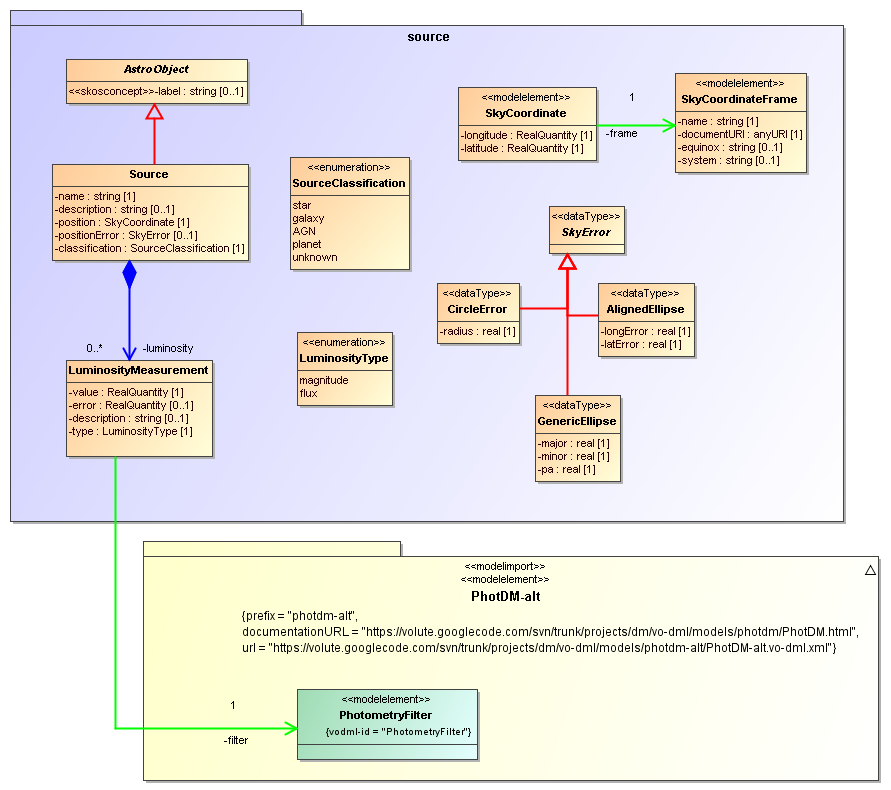
\includegraphics[width=6in,height=5.32014in]{./media/image32.png}

Figure Simple Source data model used for illustrations in this document.

\hypertarget{the-datamodel-registry-extension}{%
\section{The DataModel registry
extension}\label{the-datamodel-registry-extension}}

The Registry extension for registering a data model.

\textless?xml version="1.0" encoding="UTF-8"?\textgreater{}

\textless xs:schema
targetNamespace="http://www.ivoa.net/xml/DataModel/v1"

xmlns:xs="http://www.w3.org/2001/XMLSchema"

xmlns:vr="http://www.ivoa.net/xml/VOResource/v1.0"

xmlns:vodm="http://www.ivoa.net/xml/DataModel/v1"

xmlns:vm="http://www.ivoa.net/xml/VOMetadata/v0.1"

elementFormDefault="unqualified"

attributeFormDefault="unqualified"

version="1.0" \textgreater{}

\textless xs:annotation\textgreater{}

\textless xs:appinfo\textgreater{}

\textless vm:schemaName\textgreater DataModel\textless/vm:schemaName\textgreater{}

\textless vm:schemaPrefix\textgreater xs\textless/vm:schemaPrefix\textgreater{}

\textless vm:targetPrefix\textgreater vodm\textless/vm:targetPrefix\textgreater{}

\textless/xs:appinfo\textgreater{}

\textless xs:documentation\textgreater{}

This schema defines a type for registering data models written

in the VO-DML modelling language.

\textless/xs:documentation\textgreater{}

\textless/xs:annotation\textgreater{}

\textless xs:import namespace="http://www.ivoa.net/xml/VOResource/v1.0"

schemaLocation="http://www.ivoa.net/xml/VOResource/v1.0"/\textgreater{}

\textless xs:complexType name="DataModel"\textgreater{}

\textless xs:annotation\textgreater{}

\textless xs:documentation\textgreater{}

a VO-DML-based data model.

\textless/xs:documentation\textgreater{}

\textless xs:documentation\textgreater{}

In addition to usual resource metadata, this defines the

Prefix and the URI at which to retrieve the formal data

model definition.

DataModels should have IsSupplementTo relationships to their

definining standard.

\textless/xs:documentation\textgreater{}

\textless/xs:annotation\textgreater{}

\textless xs:complexContent\textgreater{}

\textless xs:extension base="vr:Resource"\textgreater{}

\textless xs:sequence\textgreater{}

\textless xs:element name="capability" type="vr:Capability"

minOccurs="0" maxOccurs="unbounded"\textgreater{}

\textless xs:annotation\textgreater{}

\textless xs:documentation\textgreater{}

a description of a capability in connection

with the data model.

\textless/xs:documentation\textgreater{}

\textless xs:documentation\textgreater{}

This could include validators, online

converters, or similar facilities.

\textless/xs:documentation\textgreater{}

\textless/xs:annotation\textgreater{}

\textless/xs:element\textgreater{}

\textless xs:element name="dm-prefix" type="xs:string"

minOccurs="1" maxOccurs="1"\textgreater{}

\textless xs:annotation\textgreater{}

\textless xs:documentation\textgreater{}

the prefix clamined by the datamodel, including a

training colon.

\textless/xs:documentation\textgreater{}

\textless xs:documentation\textgreater{}

Each data model can only claim one prefix. Before

claiming a prefix, a search in the VO Registry must

ascertain that the prefix is not claimed by another

data model.

\textless/xs:documentation\textgreater{}

\textless/xs:annotation\textgreater{}

\textless/xs:element\textgreater{}

\textless xs:element name="dm-uri" type="xs:string"

minOccurs="1" maxOccurs="1"\textgreater{}

\textless xs:annotation\textgreater{}

\textless xs:documentation\textgreater{}

The URI of the VO-DML definition of the data

model.

\textless/xs:documentation\textgreater{}

\textless xs:documentation\textgreater{}

This URI should be constant by major version of

the standard; see the VO-DML REC for deployment

advice.

\textless/xs:documentation\textgreater{}

\textless/xs:annotation\textgreater{}

\textless/xs:element\textgreater{}

\textless/xs:sequence\textgreater{}

\textless/xs:extension\textgreater{}

\textless/xs:complexContent\textgreater{}

\textless/xs:complexType\textgreater{}

\textless/xs:schema\textgreater{}

\hypertarget{sample-vodmldatamodel-record-for-the-ivoa-model}{%
\section{Sample vodml:DataModel record for the ivoa
model}\label{sample-vodmldatamodel-record-for-the-ivoa-model}}

The following is an example of a vodm:DataModel registry record. Such
records are used to claim VODML prefixes and associate them with DM
URIs. The example is written to match the ivoa base model defined in
section 5 . Note that the record for the model that is actually in the
VO Registry may be different from this.

\textless!-\/- A registry record defining the \uline{ivoa} data model
contained in this

standard -\/-\textgreater{}

\textless ri:Resource

xsi:type=\emph{"vodm:DataModel"}

created=\emph{"2017-07-24T09:00:00"}

updated=\emph{"2017-07-24T09:00:00"}

status=\emph{"active"}

xmlns:vr=\emph{"http://www.ivoa.net/xml/VOResource/v1.0"}

xmlns:vodm=\emph{"http://www.ivoa.net/xml/DataModel/v1"}

xmlns:xsi=\emph{"http://www.w3.org/2001/XMLSchema-instance"}

xmlns:ri=\emph{"http://www.ivoa.net/xml/RegistryInterface/v1.0"}

xsi:schemaLocation=\emph{"http://www.ivoa.net/xml/VOResource/v1.0}

\emph{http://www.ivoa.net/xml/VOResource/v1.0}

\emph{http://www.ivoa.net/xml/DataModel/v1}

\emph{http://www.ivoa.net/xml/DataModel/v1}

\emph{http://www.ivoa.net/xml/VOResource/v1.0}

\emph{http://www.ivoa.net/xml/VOResource/v1.0}

\emph{http://www.ivoa.net/xml/RegistryInterface/v1.0}

\emph{http://www.ivoa.net/xml/RegistryInterface/v1.0}

\emph{"}\textgreater{}

\textless title\textgreater The \uline{ivoa} data
model\textless/title\textgreater{}

\textless identifier\textgreater{}\uline{ivo}://ivoa.net/\uline{std}/\uline{ivoadm}\textless/identifier\textgreater{}

\textless curation\textgreater{}

\textless publisher\textgreater IVOA\textless/publisher\textgreater{}

\textless creator\textgreater\textless name\textgreater{}\uline{Lemson},
G.\textless/name\textgreater\textless/creator\textgreater{}

\textless creator\textgreater\textless name\textgreater{}\uline{Laurino},
O.\textless/name\textgreater\textless/creator\textgreater{}

\textless creator\textgreater\textless name\textgreater{}\uline{Bourges},
L.\textless/name\textgreater\textless/creator\textgreater{}

\textless creator\textgreater\textless name\textgreater{}\uline{Cresitello}-\uline{Dittmar},
M.\textless/name\textgreater\textless/creator\textgreater{}

\textless creator\textgreater\textless name\textgreater{}\uline{Demleitner},
M.\textless/name\textgreater\textless/creator\textgreater{}

\textless creator\textgreater\textless name\textgreater{}\uline{Donaldson},
T.\textless/name\textgreater\textless/creator\textgreater{}

\textless creator\textgreater\textless name\textgreater{}\uline{Dowler},
P.\textless/name\textgreater\textless/creator\textgreater{}

\textless creator\textgreater\textless name\textgreater Graham,
M.\textless/name\textgreater\textless/creator\textgreater{}

\textless creator\textgreater\textless name\textgreater Gray,
N.\textless/name\textgreater\textless/creator\textgreater{}

\textless creator\textgreater\textless name\textgreater{}\uline{Michel},
L.\textless/name\textgreater\textless/creator\textgreater{}

\textless creator\textgreater\textless name\textgreater{}\uline{Salgado},
J.\textless/name\textgreater\textless/creator\textgreater{}

\textless!-\/- this should be the date of the last recommendation
-\/-\textgreater{}

\textless date
role=\emph{"update"}\textgreater2017-09-25\textless/date\textgreater{}

\textless version\textgreater1.0\textless/version\textgreater{}

\textless contact\textgreater{}

\textless name\textgreater IVOA Data Models
WG\textless/name\textgreater{}

\textless email\textgreater{}\uline{dm@ivoa.net}\textless/email\textgreater{}

\textless/contact\textgreater{}

\textless/curation\textgreater{}

\textless content\textgreater{}

\textless subject\textgreater Virtual
observatory\textless/subject\textgreater{}

\textless description\textgreater{}

Ultimately all types in a VO-DML model are defined as hierarchies

of primitive types. This Model defines a special, predefined model

that contains a set of the most common of such types: integer,

real, string etc. This

\textless/description\textgreater{}

\textless referenceURL\textgreater http://ivoa.net/documents/VODML/\textless/referenceURL\textgreater{}

\textless type\textgreater Other\textless/type\textgreater{}

\textless contentLevel\textgreater Research\textless/contentLevel\textgreater{}

\textless relationship\textgreater{}

\textless relationshipType\textgreater isSupplementTo\textless/relationshipType\textgreater{}

\textless relatedResource ivo-id=\emph{"ivo://ivoa.net/std/VODML"}

\textgreater VO-DML: a consistent modeling language for IVOA data

models\textless/relatedResource\textgreater{}

\textless/relationship\textgreater{}

\textless/content\textgreater{}

\textless dm-prefix\textgreater{}\uline{ivoa}\textless/dm-prefix\textgreater{}

\textless dm-uri\textgreater http://www.ivoa.net/dm/ivoa.vo-dml.xml\textless/dm-uri\textgreater{}

\textless/ri:Resource\textgreater{}

\hypertarget{change-log}{%
\subsection{Change log}\label{change-log}}

\textbf{Version 20161222}

\begin{itemize}
\item
  Added this changelog
\item
  Added \textbackslash- to the ModelName definition
\item
  Renamed and updated section on registering and referring to data
  models based on discussions with registry chair.
\item
  Moved IVOA model from appendix to normative section 5
\end{itemize}

\textbf{Version 20170507}

\begin{itemize}
\item
  Updated section 6.2 after comments from registry chair
\item
  Added uri attribute to Model.
\item
  Added various references
\end{itemize}

\textbf{Version 20170925}

\begin{itemize}
\item
  Updated urls to only have major version.
\item
  Changed reference to mapping model to "in progress", referring to DM
  WG page.
\item
  Proposal text by Markus Demleitner's used for sections 6.1 and 6.2
\item
  Added proposed registry extension in Appendix F and sample registry
  record for the ivoa model in appendix G
\item
  Appendix E contains the registry record for the VO-DML standard
  itself.
\end{itemize}

\textbf{Version 20180227}

\begin{itemize}
\item
  Updated URLs, removing references to volute documents, pointing where
  required to a landing page on the IVOA-wiki
\item
  Changed text on rational and complex to conform to them becoming
  primitive types
\end{itemize}

\textbf{Version 20180505}

\begin{itemize}
\item
  Added explicit statement regarding case-sensitivity of vodml-id and
  vodml-ref.
\item
  Various fixes of types, restatements to make things clearer and other
  changes inspired by the TCG comments on the RFC page.
\end{itemize}
\end{document}